\cleardoublepage
\section{TODO}
\vspace{7.5cm}

\sbnote{For the glossary, double-check your definitions with those you find in Section 2.1 in https://nvlpubs.nist.gov/nistpubs/SpecialPublications/NIST.SP.800-57pt1r5.pdf}

\sbnote{add this security property
	unlinkability: "for two observed values, the adversary cannot distinguish between a protocol execution in which they belong to the same user and a protocol execution in which they belong to two different users."
}

\url{https://www.cybok.org/media/downloads/Formal_Methods_for_Security_v1.0.0.pdf}
\url{https://cryptobook.nakov.com/asymmetric-key-ciphers/ecies-public-key-encryption}
\url{https://www.ncsc.gov.uk/whitepaper/advanced-cryptography}
\url{https://blog.cloudflare.com/post-quantum-key-encapsulation/}
\url{https://berry.win.tue.nl/CryptographicProtocols/LectureNotes.pdf}
\url{https://asecuritysite.com/}
\url{https://cryptography101.ca/}


* to symmetric encryption, add lightweight nist crypto ciphers like ascon aead 128 and https://eprint.iacr.org/2024/1618




aggiungi "accountability" nel hanbook



\sbnote{TODO In \Cref{sec:diffie_hellman}}:
* \sbnote{investigate \gls{kci}, \gls{uks} and replay attacks against 3DH? investigate also deniability (also for standard DH modes)?}
* \sbnote{what about \gls{kci} for \gls{x3dh}? check out \url{https://moderncrypto.org/mail-archive/messaging/2018/002507.html}}
* \sbnote{check out post quantum x3dh: \url{https://signal.org/docs/specifications/pqxdh/} but also \url{https://tprest.github.io/pdf/slides/x3dh-pqnet-2021.pdf} and \url{https://keitaro-hashimoto.jp/assets/pdf/PKC-HKKP21.pdf}}
* \sbnote{another interesting read for x3dh: \url{https://www.cs.ru.nl/bachelors-theses/2021/Ferran_van_der_Have___4104145___The_X3DH_Protocol_-_A_Proof_of_Security.pdf}}
For X3DH, say that ``The use of long-term keys prevents \gls{uks} attacks --- assuming long-term public keys are correctly bonded to the corresponding parties --- while, at the same time, their use does not produce a cryptographic proof of the contents of their communication or the fact that they communicated --- hence, achieving deniability. Note that a malicious server could negate communication (i.e., \gls{dos}) or refuse to hand out one-time prekeys, thus weakening the guarantees of forward secrecy.''






take material from CC deliverables (except the ones you authored, e.g., DA3/CSC-D*, those you already did), link: \url{https://drive.google.com/drive/folders/1VIRFKrMnmkf_lCf8Dei1Y7XQm2jq3QPv?usp=drive_link}


see \url{https://www.decifris.it/koine/vol4}









qui sotto commentati, link a materiale forse utile (in teoria su security of cryptographic protocols)
%* https://cseweb.ucsd.edu/classes/sp05/cse208/lec-dolevyao.html
%* http://www.sti.uniurb.it/events/fosad08/slides/Lowe_FOSAD.pdf
%* https://eprint.iacr.org/2019/1393.pdf
%* https://apps.dtic.mil/sti/tr/pdf/ADA465281.pdf
%* https://iris.polito.it/retrieve/f4a950d3-95fb-4a78-bcd8-a38866e61998/AcceptedChapter.pdf
%* Handbook of Formal Analysis and Verification in Cryptography
%* Cryptographic Protocol: Security Analysis Based on Trusted Freshness
%* http://www.lsv.fr/~kremer/Cours/MPRI1011/poly-mpri-2-30-draft.pdf
%* https://inria.hal.science/hal-01090874/document
%* Serious Cryptography by Jean-Philippe Aumasson
%* Real-World Cryptography by David Wong



\subsubsection{Re-Encryption}\label{future_sec:re_encryption}
%- Proxy Re-encryption
%	- Allows a third party called proxy to alter a ciphertext which has been encrypted for one user so that it may be decrypted by another user.

%introduced by blaze_divertible_1998


\subsubsection{Post-Quantum Cryptography}\label{future_sec:post_quantum_cryptography}
%Examples of such attacks are Shor's Algorithm --- for solving problems related to prime factorization and discrete logarithms --- and Grover's Algorithm --- for accelerating brute force attacks on symmetric cryptography;

%	https://hackmd.io/@PHD/ryiV8GolP#Quantum-Cryptography
%    see https://drive.google.com/file/d/1dG3ukw_2gCp_X2l_6MPNHOsB9IQX6xGm/view
%	We have an idea of how quantum computers work or are supposed to work.  Right now, the focus is on developing algorithms that will survive when everybody has a quantum computer.  There are none.  The approach is, can we find a math problem that a quantum computer can’t solve quickly and then model an encryption algorithm after it?
%	Ideas so far
%		Lattice-Based Cryptography
%		Multi Variable Cryptography --- there is an idea that an equation with multiple variables can’t be solved quickly, but so far all current equations have failed
%		Hash-Based Cryptography
%		Code-Based Cryptography
%		Supersingular Elliptic Curve Isogeny Cryptography
%		Symmetric Key Quantum Resistance --- AES and SNOW 3G algorithms are resistant to quantum computers if we use a large enough key
%	- quantum key distribution (this is key agreemtn scheme? or key distribution/generation?)
%https://pqshield.github.io/nist-sigs-zoo/


%As of 2025, many post‑quantum proposals are KEM-based (e.g., CRYSTALS-Kyber), while no agreed-upon post‑quantum DH has emerged (Signal proposed Post-Quantum Extended Diffie–Hellman, PQXDH, which however is based on the CRYSTALS-Kyber KEM combined with ECC – usually, curve25519).



%QUANTUM COMPUTING (1)
%Quantum computing is the use of quantum phenomena such as superposition and entanglement to perform computation. […] Quantum computers are believed to be able to solve certain computational problems, such as integer factorization (which underlies RSA encryption), substantially faster than classical computers
%https://en.wikipedia.org/wiki/Quantum_computing
%Conceived by Yuri Manin (1980) and Richard Feynman (1981), quantum computing use quantum-mechanical phenomena such as superpositionand entanglement to perform operations on data. 
%Superposition refers to a combination of states we would ordinarily describe independently.  
%To make a classical analogy, if you play two musical notes at once, what you will hear is a superposition of the two notes
%Entanglement is a famously counter-intuitive quantum phenomenon describing behaviour we never see in the classical world. 
%Entangled particles behave together as a system in ways that cannot be explained using classical logic
%
%A qubit is the quantum analogue of a classical bit and can be in two states at the same time, each with a certain probability.
%An n-qubit register can be in 2^n states at the same time, each with a certain probability.
%When a function f : {0,1}^n → {0,1}^n is applied to an n-qubit register, it is simultaneously evaluated at all 2^n states. 
%However, when the n-qubit register is measured, it reverts to being in one of the 2^n states (according to its underlying probability distribution) 
%So, quantum computers are not “massively parallel machines.” 
%
%In 1994, Peter Shor discovered a very efficient (polytime) quantum algorithm for solving the following problems 
%integer factorization: RSA affected
%discrete logarithm problem: original DH affected
%elliptic curves discrete logarithm problem: ECDH affected
%
%This implies that all RSA, DH, and ECDH implementations can be totally broken by quantum computers.





%SHOR’S ALGORITHM: HISTORY (1)
%In the early 1990s, public-key cryptography (like RSA) was becoming increasingly vital for secure digital communication
%Its security rested on the widely accepted computational hardness of factoring large numbers for classical computers
%While classical algorithms were improving, they still scaled poorly with increasing number size (super-polynomial complexity)
%Peter Shor, in 1994, presented a ground-breaking quantum algorithm capable of factoring large integers in polynomial time.
%The implication was clear: if a sufficiently powerful quantum computer could be built, the foundation of much of modern cryptography would be compromised.
%
%Key Elements of Shor's Approach
%Quantum Computation: Shor's algorithm leverages the unique                       capabilities of quantum computers:
%Superposition: Qubits can exist in multiple states simultaneously.
%Entanglement: Qubits can be linked in a way that their fates are intertwined.
%Quantum Fourier Transform (QFT): A highly efficient quantum algorithm for finding periodicity.
%Modular Arithmetic: Shor's algorithm exploits mathematical properties of modular arithmetic.
%The Essence of the Insight
%Shor's key insight was that the factors of a number N are related to the period of a certain function
%Modular Exponentiation: Consider the function: f(x) = a^x mod N, where a is a random number coprime to N.
%This function is periodic, meaning its values repeat after a certain interval.
%The period of this function is the smallest positive integer r such that a^r ≡ 1 (mod N). This r is also called the order of a modulo N.
%
%The function f(x) = a^x mod N is periodic because the possible remainders when dividing by N are finite.  Fermat's Little Theorem guarantees that   a^(N-1) ≡ 1 (mod N).  The function values will eventually repeat, and the order of 'a' modulo N determines the length of the period.

%How Periodicity Helps in Factoring
%Finding Factors from the Period: If we can find the period r, and r is even, then with a good probability, we can factor N.
%Specifically, if r is even and a^(r/2) ≠ -1 (mod N), then the greatest common divisors gcd(a^(r/2) - 1, N) and gcd(a^(r/2) + 1, N) give us non-trivial factors of N.
%Example
%Let N = 15 and a = 7.
%The function is f(x) = 7^x mod 15.
%The values are f(1) = 7, f(2) = 4, f(3) = 13, f(4) = 1, f(5) = 7 and thus the period is r = 4.
%r is even, and 7^(4/2) = 7^2 = 4 ≠ -1 (mod 15).
%gcd(7^2 - 1, 15) = gcd(48, 15) = 3
%gcd(7^2 + 1, 15) = gcd(50, 15) = 5
%The factors of 15 are 3 and 5.

%The problem reduces to find the period r
%Classically, finding the period r is computationally difficult for large N.
%Quantum Solution: Quantum Fourier Transform (QFT):
%Shor's algorithm uses the QFT to efficiently determine the period of the function.
%The QFT exploits quantum superposition and interference to reveal the periodic nature of the function.
%Intuition:
%The QFT is like a prism that decomposes a complex wave into its constituent frequencies.
%In Shor's algorithm, the function's periodicity is encoded in a quantum state, and the QFT extracts the frequency (which is related to the period).





%SHOR ALGORITHM 
%(IN A NUTSHELL)
%
% Polynomial-time quantum computer algorithm for integer factorization
%Problem: Given an integer N, find its prime factors
%Complexity: polynomial in log(N)
%Exponentially faster than the most efficient known classical factoring algorithm, the general number field sieve method
%If a quantum computer with a sufficient number of qubits could operate without succumbing to quantum noise and other quantum-decoherence phenomena, then Shor's algorithm could be used to break public-key cryptography schemes, such as the widely used RSA scheme
%Shor's algorithm shows that factoring integers is efficient on an ideal quantum computer, so it may be feasible to defeat RSA by constructing a large quantum computer
%In 2001, Shor algorithm was demonstrated on a quantum computer at IBM to factorize 15
%In 2019, 21 was factorized using Shor algorithm on a quantum computer
%
%Algorithm composed of two parts
%first turns the factoring problem into the problem of finding the period of a function (may be implemented classically) 
%second finds the period using the quantum Fourier transform (responsible for the quantum speedup)




%POST QUANTUM CRYPTOGRAPHY (PQC)
%
%Design cryptosystems based on mathematical problems that are                              not solvable by Shor algorithm
%There are several possible alternatives
%Lattices 
%Error-correcting codes 
%Multivariate polynomials 
%Hash functions 
%Elliptic curve isogenies 
%… 
%Since 2015, NIST is actively researching new, quantum-resistant algorithms to improve and extend its official standards which are binding for all federal entities, including Digital signatures and Key exchange protocols
%
%Bounded-error quantum polynomial time (BQP) is the class of decision problems solvable by a quantum computer in polynomial time, with an error probability of at most 1/3 for all instances
%
%Arbitrary value, complexity class does not change if we take exponentially small values in the size of the input





%CONJECTURED QUANTUM-SECURE PROBLEMS 
%
%Solving multivariate quadratic equations 
%Multivariate Crypto 
%Bounded-distance decoding (BDD) 
%Code-based crypto 
%Short(est) and close(st) vector problem  
%Lattice-based crypto 
%Breaking security of symmetric primitives (SHA-x-, AES-,... problem)
%Hash-based signatures / symmetric crypto 
%
%For an introduction, see the book at
%https://www.e-reading-lib.com/bookreader.php/135832/Bernstein,_Buchmann,_Dahmen_-_Post_Quantum_Cryptography.pdf 




%NIST: REQUIREMENTS ON PQC
%
%Public-key encryption: shall include algorithms for key generation, encryption, and decryption 
%Bottom line, the scheme shall support the encryption and decryption of messages that contain symmetric keys of length at least 256 bits 
%Key encapsulation mechanism (KEM): shall include algorithms for key generation, encapsulation, and decapsulation. 
%Bottom line, KEM shall support the establishment of shared keys of length at least 256 bits
%Digital signature: shall include algorithms for key generation, signature generation and signature verification 
%The scheme shall be capable of supporting a message size up to 2^(63) bits


%NIST: SECURITY LEVELS
%Any attack that breaks the relevant security definition must require computational resources comparable to or greater than those required for
%
%key search on a block cipher with a 128-bit key (e.g., AES128)
%collision search on a 256-bit hash function (e.g., SHA256/SHA3-256) 
%key search on a block cipher with a 192-bit key (e.g., AES192)
%collision search on a 384-bit hash function (e.g., SHA384/SHA3-384) 
%key search on a block cipher with a 256-bit key (e.g., AES 256) 



%NIST SELECTION PROCESS (SO FAR)
%NIST solicited proposals for quantum-resistant signature and key encapsulation algorithms. 
%November 30, 2017: 69 submissions in Round 1.
%January 30, 2019: 26 submissions selected for Round 2.
%July 22, 2020: 7+8 submissions selected for Round 3. 
%July 5, 2022: Key encapsulation scheme Kyber, and signature schemes Dilithium, Falcon, SPHINCS+ chosen for standardization.
%On August 13, 2024, NIST published the standards FIPS 203 (Kyber), FIPS 204 (Dilithium), and FIPS 205 (SPHINCS+). 
%FIPS 206 for Falcon is expected to be completed in a year or two
%More details on these can be found at 
%https://csrc.nist.gov/projects/post-quantum-cryptography/ 




%SELECTION & CRYPTO AGILITY
%In 2022, one of the algorithms selected for further study was SIKE (Supersingular Isogeny Key Encapsulation)
%SIKE is a key encapsulation (KEM) algorithm based upon a fundamentally different approach (Supersingular Isogeny) than the lattice-based Kyber algorithms chosen for KEM applications 
%Researchers at KU Leuven have published a paper (Full details at https://eprint.iacr.org/2022/975  ) claiming they were able to find an efficient key recovery attack for using a single core processor in about one hour’s time with Magma
%This led to dropping SIKE from further consideration for PQC standardization
%This certainly makes the case for using crypto-agility so algorithms can be changed out easily if a problem is found




%NIST FINAL ALGORITHMS IN A NUTSHELL
%(2024)
%
%TABELLA
%Algorithm
%Type
%Key Features
%
%CRYSTALS-Kyber
%Public Key Encryption (KEM)
%Fast key exchange, small key sizes, lattice-based security.
%
%CRYSTALS-Dilithium
%Digital Signatures
%Lattice-based, efficient signing & verification, strong security.
%
%Falcon
%Digital Signatures
%Compact signatures, optimized for constrained environments.
%
%SPHINCS+
%Hash-Based Signatures
%Stateless, post-quantum secure, higher signature size.



%TECHNICAL DETAILS & STRENGTHS (1) 
%
%CRYSTALS-Kyber (Key Encapsulation Mechanism - KEM)
%Replaces RSA/ECC for secure key exchange
%Based on structured lattices (Learning With Errors - LWE problem)
%Small key sizes compared to other PQC candidates (~1-2 KB)
%Fast encryption & decryption speeds – suitable for large-scale deployment.
%Use Case: TLS 1.3 for secure web traffic encryption, VPNs, secure messaging.
%
%CRYSTALS-Dilithium (Digital Signatures)
%Based on lattice cryptography (Module Learning With Errors - MLWE problem)
%Faster signature generation & verification than traditional RSA/ECC
%Highly resistant to quantum attacks and classical side-channel attacks.
%
%Use Case: Securing financial transactions, digital identity verification, smart contracts.
%
%Falcon (Digital Signatures)
%Based on lattice cryptography (NTRU problem)
%Smaller signature sizes than Dilithium (~500 bytes vs. 2KB)
%Requires floating-point arithmetic, making implementation more complex.
%
%Use Case: Lightweight devices, embedded systems, and IoT security.
%
%SPHINCS+ (Hash-Based Signatures)
%Based on  hash functions (instead of lattices) – resistant to all known quantum attacks
%Stateless, meaning no requirement for secure key storage
%Larger signature sizes (~40 KB) compared to Falcon and Dilithium.
%
%Use Case: Long-term data integrity & secure archival signatures (e.g., financial records, legal documents).


%PQC ADOPTION: 
%SOME ONGOING INITIATIVES
%Google: https://cloud.google.com/security/resources/post-quantum-cryptography
%Threat model and suggestions for selecting primitives for various use cases
%https://bughunters.google.com/blog/5108747984306176/google-s-threat-model-for-post-quantum-cryptography 
%Tink: an open-source cryptography library written by cryptographers and security engineers at Google
%https://developers.google.com/tink 
%AWS: https://aws.amazon.com/it/security/post-quantum-cryptography/ 
%AWS Libcrypto (AWS-LC): https://github.com/aws/aws-lc/blob/main/crypto/fipsmodule/PQREADME.md 
%s2n-tls is an implementation of the TLS/SSL protocol with PQC support: https://github.com/aws/s2n-tls 
%Apple iMessage goes PQC
%https://security.apple.com/blog/imessage-pq3/ 
%Signal also goes PQC
%https://signal.org/blog/pqxdh/ 
%…




\subsubsection{Randomness}\label{future_sec:randomness}

%\footnote{While ``random'' denotes (sequences of) values inherently unpredictable and non-deterministic --- often arising from physical processes such as radioactive decay and thermal noise --- ``pseudoranom'' denotes (sequences of) values produced by deterministic algorithms that \textit{mimic} the statistical properties of true randomness. In other words, while truly random sequences have no pattern or reproducible rule that can predict future values, pseudorandom sequences are completely determined by an initial value called \textbf{seed}. Intuitively, true randomness is complex to achieve and needs dedicated hardware support, hence pseudorandomness --- when deemed secure enough for use --- is often employed as a more usable alternative. For more details, see \Cref{future_sec:randomness}.}

%	Pseudo-random generators are more practical to use, and more popular
%   Statistical tests to check randomness: can only prove non-randomness, no finite number of tests can prove randomness.
%	The security strength of cryptographic keys can be measured as "bits of security" as
%	described in the documentation of NIST (see https://www.nist.gov/news-events/news/2020/06/cryptographic-key-generation-nist-publishes-sp-800-133-rev-2)
%	https://kel.bz/post/entropy/



%
%What is a random number generator?
%Simple answer: a device that generates sequences of numbers that look random
%What does it mean for a sequence of numbers to look random?
%To be considered truly random, a sequence of numbers must exhibit the following two properties: 
%Uniform Distribution
%All the numbers in a designated range must occur equally often 
%Independence
%Even if one knows some or all the numbers up to a certain point in a random sequence, he/she should not be able to predict the next one (or any of the future ones) 
%Truly random numbers can only be generated by physical phenomena
%Examples: thermal noise, cards, dice, …
%Computers try to approximate (simulate) truly random numbers through a variety of approaches

%A pseudorandom sequence produced by a PRNG can be made more cryptographic secure by restarting the sequence with a different seed after every N numbers
%One way to do this would be to take the current clock time modulo m as a new seed after a given numbers of the sequence have been produced

%Cryptographically secure PRNGs should hold up well under serious attacks, even when part of their initial or running state becomes available to an attacker
%This is indeed not the case of linear congruential generators considered above
%Additionally, a cryptographically secure PRNG should have additional properties that make it suitable for use in cryptographic applications including the generation of 
%nonces: for which, the crucial requirements is uniqueness
%keys: for which, the crucial requirement is entropy (i.e.  randomness collected by an operating system often collected from hardware sources such as variance in fan noise or HDD)

%The Linux kernel generates entropy keyboard timings, mouse movements, and IDE timings and makes the random data available to other operating system processes through the special files /dev/random and /dev/urandom

%More details on weaknesses of real world cryptographically secure PRNGs can be found in
%https://link.springer.com/content/pdf/10.1007/3-540-69710-1_12.pdf 

%\newglossaryentry{Entropy} {
	%	name=Entropy,
	%	description={The measure of randomness or unpredictability in the generation of cryptographic keys}
	%} ensuring the keys are resistant to statistical and computational attacks.



%LOW ENTROPY IN KEYS (1)
%	
%	The entropy of a random number generator is at its highest if all numbers are equally likely to be produced within the range of numbers that the output is designed for
%	Example
%	if a generator can produce 512-bit random numbers with equal probability, its entropy is at its maximum and it equals 512 bits
%	If the probabilities associated with the output random numbers are nonuniform, the entropy will be less than 512 bits
%	The greater the nonuniformity of the probability distribution, the smaller the entropy
%	The entropy is zero for deterministic output
%	
%	In a Usenix 2012 paper (available at https://www.usenix.org/conference/usenixsecurity12/technical-sessions/presentation/heninger), it was experimentally shown how to harvest over 5 million TLS/SSL certificates and around 4 million RSA-based SSH host keys with scanning for two days the Internet ports
%	By using appropriate algorithms, the authors were able to find the factors that any of the moduli shared with any of the other moduli from the collected keys
%	They were able to compute the private keys for
%	0.50% of the TLS/SSL servers (around 25,000)
%	0.03% of the SSH servers (around 1,200)
%	This implies that random number generators used in key generation should have high enough entropy so that every modulus is unique vis-a-vis the moduli used by any other communication device anywhere on earth
%
%	While the prescription above is followed by most computers that we currently use, this is not the case for a large number of (so called) headless communication devices such as routers, firewalls, server management cards, etc
%	A very large number of these devices use inadequate software sources of entropy for the random bytes needed to generate prime numbers
%	The problem with such software sources of entropy is at boot time when they are initialized
%	as they are not very well equipped to supply high-entropy random bytes 
%	at the same time, the network interface needs to create keys




%There are two principal methods used to generate random numbers
%The former measures some physical phenomenon that is expected to be random and then compensates for possible biases in the measurement process
%Example sources include thermal noise and other electromagnetic and quantum phenomena
%The speed at which entropy can be obtained from natural sources is dependent on the underlying physical phenomena being measured 
%Sources of naturally occurring "true" entropy are said to be blocking, i.e. measures are allowed only after enough entropy is harvested to meet the demand
%For instance, on some Unix-like systems, including most Linux distributions, the pseudo device file /dev/random will block until sufficient entropy is gathered from device drivers and other sources of environmental noise to seed a cryptographically secure pseudorandom number generator (CSPRNG)
%The second method is to use PRNGs…
%
%There are two principal methods used to generate random numbers, contd
%The second method is to use PRNGs, i.e. computational algorithms that can produce long sequences of apparently random results, which are in fact completely determined by a shorter initial value, known as a seed value or key
%Interestingly, the entire seemingly random sequence can be reproduced if the seed value is known
%This type of generator is non blocking as it typically does not rely on sources of naturally occurring entropy, though it may be periodically seeded by natural sources
%While a pseudorandom number generator based solely on deterministic logic can never be regarded as a "true" random number source in the purest sense of the word, in practice they are generally sufficient even for demanding security-critical applications
%Carefully designed and implemented pseudorandom number generators can be certified for security-critical cryptographic purposes and are called  cryptographically secure pseudorandom number generators (CSPRNGs)

%Cryptographically secure pseudorandom number generator (CSPRNG)
%It is a pseudorandom number generator (PRNG) with properties that make it suitable for use in cryptography
%Such properties depend on the use case scenario including
%key generation
%nonces
%For example, creating a nonce in some protocols requires only uniqueness
%On the other hand, the generation of a master key requires more entropy
%In the case of one-time pads, the information-theoretic guarantee of perfect secrecy only holds if the key material comes from a true random source with high entropy, and thus any kind of pseudorandom number generator is insufficient
%Ideally, the generation of random numbers in CSPRNGs uses entropy obtained from a high-quality source, generally the operating system's randomness API
%Unexpected correlations have been found in several such ostensibly independent processes
%
%For the details underlying
%one CSPRNG used in 
%real applications, see
%https://www.schneier.com/wp-content/uploads/2015/12/fortuna.pdf 

%CSPRNG designs can be based on cryptographic primitives
%A secure block cipher can be converted into a CSPRNG by running it in counter mode using, for example, a special construct that the NIST calls CTR_DRBG that typically uses AES
%The NIST CTR_DRBG scheme erases the key after the requested randomness is output by running additional cycles. This is wasteful from a performance perspective, but does not immediately cause issues with forward secrecy
%Full details available at https://csrc.nist.gov/pubs/sp/800/90/a/r1/final 
%A stream cipher, such as RC4 or ChaCha20, can be converted into a CSPRNG
%A hash and a HMAC can also be used as a base of a CSPRNG
%CSPRNG designs can also be based on mathematical problems thought to be hard including the Blum Blum Shub algorithm, Blum–Micali algorithm, and  Dual EC DRBG 
%The last algorithm was presented as a CSPRNG using methods in elliptic curve cryptography. Despite wide public criticism, including the public identification of the possibility that the NSA put a backdoor into a recommended implementation, it was, for seven years, one of four CSPRNGs standardized by as originally published circa June 2006, until it was withdrawn in 2014

%"Practical" CSPRNG schemes not only include an CSPRNG algorithm, but also a way to initialize ("seed") it while keeping the seed secret
%A number of such schemes have been defined, including:
%Implementations of /dev/random in Unix-like systems
%Yarrow, which attempts to evaluate the entropic quality of its seeding inputs, and uses SHA-1 and 3DES internally. Yarrow was used in macOS and other Apple OS' up until about December 2019, after which it switched to Fortuna
%Fortuna, the successor to Yarrow, which does not attempt to evaluate the entropic quality of its inputs; it uses SHA-256 and "any good block cipher". Fortuna is used in FreeBSD. Apple changed to Fortuna for most or all Apple OSs beginning around Dec. 2019.
%The Linux kernel CSPRNG, which uses ChaCha20 to generate data and BLAKE2s to ingest entropy
%arc4random, a CSPRNG in Unix-like systems that seeds from /dev/random, originally based on RC4, but all main implementations now use ChaCha20


\subsubsection{Cryptographic Accumulators}\label{future_sec:cryptographic_accumulators}


\subsubsection{Cryptographic Ratchets}\label{future_sec:cryptographic_ratchets}

%\sbnote{see \url{https://signal.org/docs/specifications/doubleratchet/} and \url{https://signal.org/docs/specifications/sesame/}}

%		Description: ratcheting* mechanisms ensure that cryptographic protocols can recover from key compromise over time – that is, post-compromise security (PCS);
%		relevance: an attacker that obtains currently used private or secret keys may decrypt all future messages. Ratcheting mechanisms allow cryptographic protocols to self-heal after compromise – that is, once the attacker is out of the loop, future messages become secure again;
%		attacks mitigated: long-term confidentiality violation attacks (mitigation only);
%		additional considerations: the Signal cryptographic protocol employs a double ratchet algorithm. Ratcheting mechanisms usually occurs in place of full key renegotiation (which may be computationally demanding and slower).
%		
%		*Ratcheting involves continuously evolving cryptographic keys in a forward-only fashion, such that each new key is derived from the previous one, usually with input from fresh entropy or messages. This ensures forward secrecy and additionally introduces backward secrecy (also known as self-healing): if attackers compromise a device and learn its current key material, they can only decrypt a limited number of past/future messages.

\subsubsection{Other Stuff}\label{sec:TEMPORARY_LABEL:minor}
\begin{itemize}
	\item add birthday paradox to glossary
	\item Key Clustering
	\item (Key) Diffusion and (Key) Confusion
	%	§ Diffusion
	%	If a plaintext bit changes, several ciphertext bits should change
	%	§ This is a basic demand on a block cipher, and ensures that the statistics used
	%	are block statistics
	%	§ This is typically achieved by using linear transformations (e.g., shifting bits)
	%	§ Confusion
	%	Every bit of the ciphertext should depend on several bits in the key
	%	§ This can be achieved by ensuring that the system is nonlinear 
	%			As Shannon suggested, diffusion and confusion are fundamental properties for both hashing and symmetric cryptography
	%			- for the former, linear functions (such as shifting, a bit level manipulation) can be used
	%			- for latter, non linear functions (such as addition modulo, that can be implemented efficiently with bit level manipulations or substitutions by using constants, that can be efficiently implemented by array operations) shall be used 
	%			- non linear transformations are used in combination with linear ones to make the latter less predictable
	\item message- or key-commitment
	%	Most ciphers are not “committing”. This means that a single ciphertext can be decrypted (using different keys) to different valid plaintexts. This is true even for AEAD ciphers such as AES-GCM and chacha20/poly1305. AES-GCM not being committing
	\item Onion encryption
	\item Key splitting (vs. key sharing)
	\item Blind signatures
	%	=> Ability to sign documents without knowledge of content, similar to a notary public.
	\item Digital Signature Standard (DSS)
	%		https://nvlpubs.nist.gov/nistpubs/FIPS/NIST.FIPS.186-4.pdf
	\item protocols like OTR (Off-the-Record)
	\item Key distribution with trusted third party/key distribution center (KDC) - KDC may have hierarchies for large networks
	%	=> for instance: kerberos (mention also needham schroeder) = da slide 21 in https://drive.google.com/file/d/1md3iVwPwy5rgwcy5HDqPULAo6R7i4kjo/view
	%	\item Authenticated Key Exchange (AKE)
	%	High-level concept of using an authenticity mechanism (e.g., MAC, digital signature) with a KEM — often through the use of DH. For instance, TLSv1.3 uses digital certificates as authenticity mechanism to sign (ephemeral) asymmetric keys used in ECDHE-AKEM — used then to derive symmetric keys.
	\item Password-Authenticated Key Exchange (PAKE)
	%	A specific instance of AKE. A PAKE may be:
	%	* *balanced* — that is, the two parties use the same password to negotiate and authenticate a shared key (mutually authenticated);
	%	* *augmented* — that is, one party is a prover while the other party is a verifier. Augmented PAKE is often used in client-server scenarios, so to avoid that an attacker can recover the password by compromising the server.
	%	
	%	On request of IETF, a PAKE selection process has been carried out in 2018 and 2019 by the IRTF crypto forum research group (CFRG), resulting in one balanced PAKE (CPace) and one augmented PAKE (OPAQUE). https://blog.cloudflare.com/opaque-oblivious-passwords
	\item Signcryption
	%An asymmetric cryptographic algorithm that guarantees confidentiality (e.g., encryption) as well as integrity, authenticity and non-repudiation (e.g., digital signatures).
	
	
	\item random Oracle Model
	%	We get to assume that we have access to Random Oracles (ROs). Incredibly weird and critical to cryptographic proofs, but you can just think of it like a “perfect” cryptographic hash function (possibly with variable length output). As this is an imaginary construct anyway, there are an infinite number of different ROs which each map their inputs to ourputs differently. Generally, you don’t care which you have as long as you have one. (This also means that papers might use more than one RO within the same paper for different purposes.) In security proofs both the challenger and adversary can query it and the adversary has the ability to pre-program its responses.
	
	\item Games
	%	A game is some set sequence of allowed actions between a challenger and an adversary. The majority of security definitions are given by describing a game and saying something is secure if no PPT adversary can win the game with more than negligible probability
	%	An “Adversary” is some limited (usually normal probability polynomial time) algorithm which is trying to break an algorithm. (Probabilistic polynomial time just means it can runs relatively quickly and has access to random bits.)
	%	A “Challenger” generally uses an algorithm (being proven to have certain properties) and random bits to pose some sort of challenge to an adversary in the context of a game. For example “Is this string the result of encrypting the data you gave me under a random key OR is it just completely random data?”
	
	
	\item cifrari tweakable 
	%	Un cifrario a blocco funziona normalmente in modo deterministico: dati i due in-
	%	gressi richiesti (messaggio in chiaro e chiave segreta) esso produce in uscita un
	%	messaggio cifrato che corrisponde in modo biunivoco ai due ingressi dati. Per-
	%	tanto, se si ripete la cifratura usando la medesima coppia di ingresso si ottiene
	%	in uscita il medesimo messaggio cifrato. Questa è una proprietà utile al progetto
	%	ed all’analisi del cifrario, ma che diventa deleteria quando lo si utilizza in pratica.
	%	Infatti, è facile verificare che tale funzionamento deterministico non consente di
	%	avere sicurezza nello scenario CPA (Chosen Plaintext Attack), requisito basilare
	%	della cifratura simmetrica.
	%	Partendo da un cifrario a blocco deterministico (come AES), si vuole pertan-
	%	to rendere l’output della cifratura aleatorio, ovvero variabile in modo casuale ad
	%	ogni cifratura, pur mantenendo fissi il messaggio in chiaro e la chiave segreta.
	%	Ciò normalmente si ottiene ricorrendo alle cosiddette modalità operative, ossia
	%	CloudCiphers
	%	3
	%	Standard NIST per FPE
	%	Univpm
	%	11R4-UnivPM-D1-def
	%	costruzioni algoritmiche che incorporano un cifrario a blocco deterministico e
	%	mescolano i suoi ingressi ad una stringa pseudo-casuale che varia ad ogni invo-
	%	cazione del cifrario stesso. Tale stringa assume un valore iniziale detto anche
	%	vettore di inizializzazione (IV), che viene scelto in modo pseudo-casuale da chi
	%	cifra (Alice) e trasmesso in chiaro a chi decifra (Bob). Non è infatti necessaria
	%	la confidenzialità del vettore di inizializzazione, il quale non concorre alla confi-
	%	denzialità del testo in chiaro né della chiave, ma ha soltanto lo scopo di rendere
	%	aleatorio il testo cifrato.
	%	Un’alternativa all’uso delle modalità operative e del relativo vettore di inizia-
	%	lizzazione consiste nell’uso dei cifrari a blocco detti “tweakable”, introdotti da
	%	Liskov, Rivest e Wagner nel 2011 [22]. Un cifrario tweakable, oltre al messaggio
	%	in chiaro ed alla chiave segreta, riceve in ingresso un terzo valore, detto appunto
	%	“tweak”. Quest’ultimo ricopre la stessa funzione di un vettore di inizializzazione
	%	per le modalità operative, alterando il legame tra gli altri ingressi e l’uscita del
	%	cifrario, con la differenza che tale funzione è incorporata direttamente nel cifra-
	%	rio, anziché basarsi su una costruzione superiore come nel caso delle modalità
	%	operative.
	%	Il tweak è pensato per poter essere cambiato frequentemente, quindi cambia-
	%	re il valore del tweak deve essere una operazione efficiente, non deve richiedere
	%	di modificare la chiave e deve costare meno che cambiare la chiave. Per quanto
	%	riguarda la sicurezza, anche se un attaccante può controllare il valore del tweak,
	%	il cifrario deve rimanere sicuro, e questo si ottiene se ogni scelta del valore del
	%	tweak produce un comportamento del cifrario diverso e indipendente dagli altri.
	
	
	\item Format-Preserving Hash (FPH)
	
	
	
	\item qualified digital signatures
	%	FIRME DIGITALI QUALIFICATE
	%	
	%	Digital signatures in eIDAS
	%	https://eur-lex.europa.eu/legal-content/EN/TXT/?uri=uriserv:OJ.L_.2014.257.01.0073.01.ENG
	%	
	%	
	%	(digital) electronic signature (ES) = 
	%	data in electronic form which is attached to or logically associated with other data in electronic form and which is used by the signatory to sign
	%	
	%	(digital) advanced electronic signature (AdES) = 
	%	an electronic signature with some security features that ensure it is 
	%	* uniquely linked to the signatory, it is capable of identifying the signatory 
	%	* it is linked to the data in such a manner that any subsequent change of the data is detectable
	%	
	%	(digital) qualified electronic signatures (QES) = 
	%	an advanced electronic signature which provides 
	%	* additional level of assurance on the identity of the signatory 
	%	* an enhanced protection and level of assurance on the signature creation 
	%	A special device is required for the creation of QES (a qualified signature creation device, QSCD).
	%	
	%	QSCD shall ensure
	%	(a) the confidentiality of the private key used for electronic signature
	%	creation is reasonably assured;
	%	
	%	(b) the private key used for electronic signature creation can
	%	practically occur only once;
	%	
	%	(c) the private key used for electronic signature creation cannot, with
	%	reasonable assurance, be derived and the electronic signature is reliably protected against
	%	forgery using currently available technology;
	%	
	%	(d) the private key used for electronic signature creation can be
	%	reliably protected by the legitimate signatory against use by others.
	%	
	%	
	%	A QES shall have the equivalent legal effect of a handwritten
	%	signature and shall be recognised as a qualified electronic
	%	signature in all Member States.
	%	
	%	This equivalence is gained from the fact that qualified
	%	electronic signatures are supported by
	%	i) trustworthy process technology, similar to advanced
	%	electronic signatures,
	%	ii) qualified electronic signature creation devices and
	%	iii) qualified trust service providers (QTSPs) - which are
	%	supervised by EU MS appointed supervisory bodies - that issues 
	%	(digital) qualified certificates
	%	
	%	
	%	QES should provide non-repudiation and sender authenticity
	%	QES: Signing with the same legal value as with a handwritten signature 
	%	
	%	In Europe the current framework for legally binding electronic sig-
	%	natures is based on the eIDAS Regulation from 2014 and its concept
	%	of qualified services
	%	
	%	
	%	besides QES, there are also electronic seals, which authenticate digital documents created by legal persons.
	%	electronic seals are essentially QES
	%	the technical requirements for QES apply to electronic seals
	%	
	%	Ring signatures CANNOT be QES
	%	Group signatures and pseudonymous signatures can be QES, as 
	%	it is possible to link a signature to its creator
	%	
	%	Qualified signatures are the only ones for which equivalence to the
	%	written form is satisfied
	%	
	%	
	%	Note that eIDAS does not state that for each private key
	%	there must be corresponding public key
	%	
	%	The lack of a one-to-one mapping between private key and
	%	public key is a decision that makes room for advanced
	%	solutions such as Pseudonymous Signatures
	%	The idea of Pseudonymous Signature is that a citizen keeps a single signing key
	%	on the personal identity card. Nevertheless, this cryptographic key corresponds
	%	to a potentially unlimited number of public key
	%	
	%	
	%	eIDAS and the GDPR
	%	QES are personal data, i.e., requires consent to process (e.g., validate)
	%	
	%	
	%	
	%	
	%	
	%	this stuff is evolving
	%	
	%	The EU Commission published a proposal for a number of
	%	modifications in eIDAS
	%	
	%	There is a slight change in the notion of a certificate, i.e., a certificate will be understood as a bag of
	%	atomic attestations
	%	
	%	The main revolution is the introduction of a unified European Digital
	%	Identity Wallet
	%	European Digital Identity Wallets shall enable the user to: [...] (b)sign by
	%	means of qualified electronic signatures
\end{itemize}



\sbnote{for the definition of Security Properties in Cryptography, see Section 3 Security Services of https://nvlpubs.nist.gov/nistpubs/SpecialPublications/NIST.SP.800-57pt1r5.pdf}	


\sbnote{vedi anche qui per glossary \url{https://nvlpubs.nist.gov/nistpubs/SpecialPublications/NIST.SP.800-57pt2r1.pdf}}

vedi \url{https://arxiv.org/pdf/1605.09771}

\sbnote{vedi \url{https://cryptowiki.tm.kit.edu/index.php/Main_Page}}

\sbnote{interesting: <comment>}%https://www.etsi.org/deliver/etsi_ts/119300_119399/119312/01.04.03_60/ts_119312v010403p.pdf

\sbnote{interesting 2: <comment>}%https://www.sogis.eu/documents/cc/crypto/SOGIS-Agreed-Cryptographic-Mechanisms-1.3.pdf


\sbnote{add in glossary what is commented below}
%cryptographic engineering: the selection, adaption, implementation, and roll-out of cryptographic primitives in systems, services, and applications



TO READ
%- https://www.cryptologie.net/article/504/why-im-writing-a-book-on-cryptography/
%- https://www.cryptofails.com/
%- https://www.cryptofails.com/post/75204435608/write-crypto-code-dont-publish-it
%- https://csrc.nist.gov/News/2023/lightweight-cryptography-nist-selects-ascon
%- https://csrc.nist.gov/projects/cryptographic-standards-and-guidelines/
%- https://people.cs.rutgers.edu/~pxk/419/notes/
%- https://nvlpubs.nist.gov/nistpubs/SpecialPublications/NIST.SP.800-56Ar3.pdf
%=> check whether One-Pass Unified Model is ECDHE-AKEM
%- https://www.ietf.org/archive/id/draft-ietf-mls-protocol-20.html
%=> Messaging Layer Security (MLS)
%=> TreeKEM
%- https://noiseprotocol.org/
%- https://www.crypto101.io/
%- https://textbook.cs161.org/crypto/symmetric.html
%- https://crypto.stanford.edu/~dabo/cryptobook/BonehShoup_0_6.pdf

SUBSCRIBE 
%- RED HAT
%- BLACK HAT
%- HACKER NEWS

Blog
%* Neil Madden's blog;\footnote{\url{https://neilmadden.blog/author/neilmadden/}}
%* Soatok's blog;\footnote{\url{https://soatok.blog/author/soatok/}}
%* Ryan Castellucci's blog;\footnote{\url{https://rya.nc/}}
%* kel.bz;\footnote{\url{https://kel.bz/}}
%* last article you read was on 23/08/2023: "Physical proximity and latency" (dates 28/03/2021)
%* Matthew Green's blog;\footnote{\url{https://blog.cryptographyengineering.com/}}
%* Chosen Plaintext Consulting's blog.\footnote{\url{https://www.chosenplaintext.ca/blog/}}
%* Latacora.\footnote{\url{https://www.latacora.com/blog/}}
%* https://www.telsy.com/it/home/


%* https://gist.github.com/tqbf/be58d2d39690c3b366ad
%* https://gist.github.com/atoponce/07d8d4c833873be2f68c34f9afc5a78a





UN SACCO DI ROBA COMMENTATA QUI
%Minor fixes and modifications to the content of the Crypto Handbook
%- Redefine the concept of key (e.g., a private key may also be an isogeny in post-quantum ciphers) as something like "A sequence of bits representing information known only by..."
%- "KEM" may also mean "Key Exchange Module" and not only "Key Encapsulation Mechanism"?
%- https://milagro.apache.org/cdocs/index.html
%- https://zenroom.net/
%
%best practices
%- use only secure and standardized algorithms and libraries;
%- do not prioritize backwards compatibility at the expense of security;
%- carefully read the standards and documentation when using an algorithm or library;
%- Never use a key for more than one purpose (e.g., encrypting, digital signatures, MACs);
%- Always use cryptographically secure pseudorandom number generators.
%- HMAC keys should be the same length as the hash output.
%- Rotate keys periodically
%- Some algorithms (e.g., hashes, KDF) may generate similar outputs when inputs are the same and only the length is changed
%- never reuse a nonce or IV (in a given context, usually relative to a key)
%- follow the Cryptographic Agility principle when designing a system employing cryptography
%- An attacker mustn’t be allowed to select the actual value being validated in the signature. Otherwise, they could trivially craft a valid signature for an arbitrary public key by (essentially) generating a random signature and seeing what message would be verified by that signature and then returning that message/signature pair.
%- Just because a signature is valid for a given message doesn’t mean it isn’t valid for other messages.
%- Signatures do not (necessarily) hide the message they sign. They’ll commonly reveal the hash (or more) of the data being signed.
%- Signatures do not hide the public key used to verify the message.
%
%The simplest building blocks of encryption are:
%substitution: in which each symbol is exchanged for another (not
%necessarily uniformly), and
%transposition: in which the order of symbols is rearranged.
%It might seem that these are too naive to be effective. But almost
%all modern commercial symmetric ciphers use some combination of
%substitution and transposition for encryption.
%
%Two things an encryption step can provide are:
%Confusion: transforming information in plaintext so that an
%interceptor cannot readily extract it.
%Diffusion: spreading the information from a region of plaintext
%widely over the ciphertext.
%Substitution tends to be good at confusion; transposition tends to
%be good at diffusion.
%
%textbook crypto e material
%https://www.schneier.com/books/applied_cryptography/  
%https://g.co/kgs/d7sYdH
%http://math.harvard.edu/~ctm/home/text/others/shannon/entropy/entropy.pdf
%https://sites.google.com/view/intro2cns/
%
%Per la matematica dei cifrari, un ottimo libro di testo su campi finiti e' Childs:  https://igortitara.files.wordpress.com/2010/04/a-concrete-introduction-to-higher-algebra1.pdf
%
%https://cryptocouple.com/
%
%GLOSSARY
%- generator
%- primitive root è alias per generator
%
%You will know that the message comes from them but once you know, you are in a position to be able to fake that message.
%
%But in the initial "prekey bundle" bob is sending his prekey signature, signed with his identiity key. Does this not give a proof that bob has been involved in the exchange?
%
%The definition of deniability was changed between 3DH and X3DH. X3DH provides a weaker deniability than 3DH. 3DH's deniability is that anyone can create a fake conversation. X3DH's deniability is that only people capable of being in the conversation can create a fake conversation. Note that X3DH could of been 3DH with an extra DH of signed prekey to ephemeral key and then it would of been the same deniability as 3DH.
%
%=> point is: how can you demonstrate that someone was involved in a conversation? You need to repeat the DH from this someone's point of view, i.e., using his private keys => but if ephemeral keys were used and disposed, well, it is not possible to repeat the DH.
%
%=> signature is evidence of communication and knowing of ephemeral keys, and hence knowing of SK
%
%Regarding authenticaiton
%=> binding of public keys with identities is not guaranteed by PKI in X3DH
%=> X3DH/Signal does not care, and tells to use QR codes or "safety numbers" for verification
%

\url{https://cryptobook.nakov.com/}

FOR THE NONCE, SEE \url{https://moxso.com/blog/glossary/nonce}





%\newglossaryentry{Cryptographic Agility} {
	%	name=Cryptographic Agility,
	%	description={The ability of a system to seamlessly and (and at least partially) automatically adapt to new cryptographic standards, best practices, and recommended parameters (e.g., key lengths) by swapping out or upgrading vulnerable or deprecated algorithms, ciphers and cryptosystems without compromising security or causing major disruptions to the system itself. Cryptographic agility is often called \textit{cryptoagility} or \textit{crypto-agility}.}
	%}
%





%
%\newglossaryentry{Policy} {
	%	name=Policy,
	%	description={A set of rules and requirements pertaining to a specific aspect of a system.}
	%}
%
%\newglossaryentry{Security Policy} {
	%	name=Security Policy,
	%	description={A set of declarative rules and requirements pertaining security-relevant aspects of a system and its components.}
	%}
%
%\newglossaryentry{Security Mechanism} {
	%	name=Security Mechanism,
	%	description={A device, method, or function for fulfilling security-relevant rules or achieving security-relevant requirements.}
	%}
%
%\newglossaryentry{Security Service} {
	%	name=Security Service,
	%	description={A logical capability comprising and orchestrating one or more security mechanisms for enforcing security policies. Examples of security services are key management, access control, and authentication.}
	%}
%For a use case scenario,  designers must decide what it means for the system to be secure, i.e. which security goals among confidentiality, integrity and availability should be achieved
%A description of the security goals is a security policy
%The implementation of a security policy is called a security mechanism
%So, the implementation of cryptographic primitives is a security mechanism
%Most security mechanisms and in particular cryptographic primitives are composed of two parts
%code and
%configuration, e.g. encryption keys and any other cryptographic parameter
%A security service is an entity that supports one or more security objectives
%It can be seen as a set of security mechanisms achieving different security goals at the same time
%It is typically easier to configure a security service than a security mechanism
%
%Security mechanisms and services are human made, typically software, artefacts that need to be implemented carefully to avoid vulnerabilities in them
%Indeed, a bug in the implementation of a security mechanism may allow attackers to bypass the enforcement of a security policy thus opening to the possibility of violating a security goal
%Additionally, security mechanisms and services must be suitably configured in the context of the system being protected that operates in a particular use case scenario
%In other words, not only security mechanisms should come with a high level of assurance but also they should be used in a suitable set up
%It is thus crucial to implement security mechanisms with a high level of assurance
%I.e. strong evidence for confidence that the set of security mechanisms or services in an information system are effective in their application



\sbnote{TODO talk about lattice-, code-, isogeny-based problems in \Cref{sec:mathematical_underpinnings}}




%vedi se utile
%https://drive.google.com/file/d/1P7bZcXMpmEmyen7kpNnBcfXeWhwgf3TP/view?usp=drive_link





elligator
%https://elligator.org/
%Censorship-circumvention tools are in an arms race against censors
%The censors study all traffic passing into and out of their controlled sphere, and try to disable censorship circumvention tools without completely shutting down the Internet
%Tools aim to shape their traffic patterns to match unblocked programs, so that simple traffic profiling cannot identify the tools within a reasonable number of traces; the censors respond by deploying firewalls with increasingly sophisticated deep-packet inspection
%Cryptography hides patterns in user data but does not evade censorship if the censor can recognize patterns in the cryptography itself
%Elliptic-curve cryptography often transmits points on known elliptic curves, and those points are easily distinguishable from uniform random strings of bits
%Elligator is a set of  high-security high-speed elliptic curve systems in which elliptic-curve points are encoded so as to be indistinguishable from uniform random strings



\sbnote{TODO search revocation based on Certificate Transparency (CT) logs and add it to \Cref{sec:binding_keys_to_parties:revocation}}



se è disponbile il DOI, aggiorna la reference \cite{kumar_demystifying_2025}






























\subsubsection{Post-Quantum Cryptographic Hash Functions}\label{future_sec:hash_functions:cryptographic_hash_function:post_quantum}




%	\sbnote{To decide what to do with the following sections of 
	%	key management; interesting but section on key management
	%	is already long, I would like to keep it short}
%	\subsection{Further Aspects of Key Management}\label{sec:further:key_management}

The security of cryptographic keys is not limited to just a proper definition of the functional aspects of key management (i.e., those described in \Cref{sec:key_management}) and the choice of the most suitable Cloud-based \gls{kms} services (see \Cref{sec:cloud}). Therefore, below we identify and briefly discuss further aspects relevant to the secure development and deployment of key management and \glspl{kms}.



\subsubsection{Policies}\label{sec:further:key_management:policies}

The management of cryptographic keys involves the definition, enforcement, and continuous revision of various policies --- a policy can be seen as a set of rules pertaining to a specific aspect of a system (e.g., a \gls{kms}). Organizations usually structure policies in a hierarchy, where each policy in a certain layer details the enforcement and implementation of the rules specified in the policies of the higher layer(s) \cite{barker_framework_2013}. In other words, top-level policies define security, business, and regulatory requirements deriving from the organizations themselves, best practices, and relevant standards (e.g., \gls{nist}'s), while intermediate- and low-level policies describe --- in greater detail --- suitable strategies and procedures to achieve such requirements. For instance, a high-level policy requiring to ``protect sensitive data'' may be linked to an intermediate-level policy requiring to ``encrypt sensitive data in transit and at rest'' which, in turn, may be linked to a low-level policy requiring to ``encrypt data in transit using \gls{tls} and data at rest using \gls{aes}-128 in a validated \gls{fips} 140-3 Hardware-based cryptographic module''. Policies at higher levels should be easily understandable by users (e.g., textual documents, tables, flow charts), while policies at lower levels may also be directly enforceable by automated systems. In any case, policies should always be written in a formal language for unambiguous meaning. In the context of key management, \gls{nist} defines a hierarchy of policies consisting of 3 layers \cite{barker_framework_2013}:

\begin{itemize}
	\item \textbf{information management policy}: this high-level policy expresses the security, business, and regulatory requirements of the organization on the use of (various categories of) sensitive data, the definition of responsibilities and management roles, and the need for security properties such as confidentiality, integrity, and availability. The information management policy also considers industrial best practices, relevant standards, and regulatory frameworks, and it is often complemented with a risk assessment \cite{joint_guide_2012};
	\item \textbf{information security policy}: this intermediate-level policy refines the aforementioned requirements by specifying how data is categorized, the sensitivity levels assigned to data, eventual access constraints, and the permissions to distribute to the management roles. The information security policy also identifies protections for data (e.g., encryption), taking into account the threats identified in the risk assessment previously conducted;
	\item \textbf{\gls{ckmssp}}: this low-level policy --- previously known as ``Key Management Policy'' --- specifies rules for the management of keys and metadata in each phase of the lifecycle shown in \Cref{fig:lifecycle} (e.g., installation/registration, generation, utilization, rotation), with the final goal to preserve the confidentiality, integrity, availability, and authenticity of keys and metadata \cite{barker_recommendation_2019_p2}. Intuitively, the rules within the \gls{ckmssp} need to be consistent with higher-level policies and have a clear mapping with the requirements defined by the organization. Moreover, the chosen \gls{kms} --- regardless of whether it was developed by the organization itself or an external party --- should be able to enforce the \gls{ckmssp}. Usually, a \gls{ckmssp} is composed of a policy for each phase of the key management lifecycle (e.g., key generation policy, key usage policy, key recovery policy). Furthermore, a \gls{ckmssp} is usually complemented with (at least) the following policies:
	\begin{itemize}
		\item \textbf{certificate policy}: this policy regulates all aspects associated with the management (e.g., issuance, distribution, revocation, renewal) of digital certificates, including details related to their types, lifecycle, and domains of applicability. Furthermore, a certificate policy defines the architecture and the entities that compose the \gls{pki} (e.g., accredited \glspl{ca}), their roles, and their duties. Finally, a certificate policy identifies which cryptographic ciphers to use (and their configuration) for digital certificates. For more details on certificate policies, we refer the interested reader to \cite{ford_internet_2003};
		\item \textbf{key-inventory policy}: this policy outlines guidelines and procedures for managing and maintaining an inventory of cryptographic keys (see \Cref{sec:key_management:inventory}). A key-inventory policy defines what keys and metadata should be stored in the inventory management system \cite{barker_recommendation_2020_p1}, including information on responsibilities, monitoring (e.g., for expired keys and insecure cryptographic parameters), and any specific requirements imposed by legal or regulatory frameworks. For more details on key-inventory policies, we refer the interested reader to \cite{barker_recommendation_2019_p2};
		\item \textbf{\gls{ac} policy}: this policy --- usually part of \gls{iam} (see S8-CSC-D1 in \Cref{sec:intro:scope}) --- comprises rules stating which agents can perform which actions (e.g., call for key rotation, encryption) on which of the resources (e.g., keys) maintained by the \gls{kms}. A formal representation of these rules is provided by the \gls{ac} model --- e.g., \gls{rbac} \cite{sandhu_access_1998} and \gls{abac} \cite{horwitz_toward_2002} are two models --- giving the semantics for granting or denying agents’ requests. The hardware and software entities that enforce the \gls{ac} policy based on the chosen model compose the so-called ``enforcement''. The enforcement may be either centralized --- e.g., based on a standard like \gls{xacml}\footnote{OASIS eXtensible Access Control Markup Language (XACML) TC (\url{https://www.oasis-open.org/committees/tc_home.php?wg_abbrev=xacml})} or monitors like the \gls{opa}\footnote{Open Policy Agent (\url{https://www.openpolicyagent.org/})} --- or decentralized --- hence, enforced directly through cryptographic with a \gls{cac} scheme like those in \cite{berlato_formal_2022,berlato_end_2022}. For more details on \gls{ac} policies, we refer the interested reader to \cite{nist_security_2020};
		\item \textbf{cryptographic algorithm policy}: this policy selects cryptographic algorithms, ciphers, and cryptosystems, as well as key lengths approved for use in the \gls{kms}. This selection is usually based on the requirements of the organization, industrial standards, and best practices. For more details on the cryptographic algorithm policy, see \Cref{app:ciphers};
	\end{itemize}
\end{itemize}

As a final remark, organizations operating in different scenarios (e.g., financial services, pharmaceuticals, government bodies) are likely to have different policies and rules. Furthermore, cross-organizational scenarios may expect the definition of cross-domain security policies for interoperability \cite{barker_framework_2013}.



\subsubsection{Authentication and Authorization}\label{sec:further:key_management:authn}

In line with the Zero Trust security model\footnote{Zero Trust - Glossary | CSRC (\url{https://csrc.nist.gov/glossary/term/zero\_trust})} (``never trust, always verify''), any entity performing any operation within the key management lifecycle should be properly authenticated and authorized \cite{chandramouli_cryptographic_2013}. Authentication is the process of verifying --- after having previously registered --- the (digital) identity of users, processes, devices, and agents in general when attempting to access a resource or perform a digital transaction (for more details on authentication, see S8-CSC-D1 in \Cref{sec:intro:scope}), while authorization is the process of verifying to what resources (and actions) a (usually authenticated) agent has access \cite{samarati_access_2001}; the authorization process often consists of evaluating \gls{ac} rules contained in a policy to make and then enforce \gls{ac} decisions --- e.g., grant or deny an access request. In the context of cryptographic key management, authentication and authorization are of fundamental importance. For instance, the association between a digital identity and its owner is crucial for maintaining a record of activities and data access history (see \Cref{sec:further:key_management:logging}) to guarantee accountability and identify malicious activities. Moreover, the assignment of permissions to agents --- where a permission represents the ability to perform an action over a resource (e.g., rotate a cryptographic key) --- allows for regulating (and preventing unauthorized) access, checking that all applicable constraints are satisfied, and enforcing the least privilege principle;\footnote{least privilege - Glossary | CSRC (\url{https://csrc.nist.gov/glossary/term/least\_privilege})} \gls{cac} is the natural combination of cryptographic and \gls{ac} \cite{berlato_formal_2022,berlato_end_2022}.

\sbnote{TODO talk also about SoD
%Separation of Duties: Separation of duties 
%By creating distinct duties or user types, that can only perform certain operations, there is an additional layer of security applied, since multiple users would need to be in collusion for key material to be stolen or manipulated in an inappropriate manner, and the audit trail to be erased
}

\subsubsection{Logging and Auditing}\label{sec:further:key_management:logging}

In a \gls{kms} --- and key management in general --- any event concerning or relevant to cryptographic keys (i.e., creation, access, use, transmission, creation of backups, transition among key states and phases) should be properly recorded in a log and, when necessary, in the metadata of keys as well \cite{barker_profile_2015}. Logs are usually collected in a distributed fashion but then stored in a centralized way; this approach implies both the ability to integrate logs coming from different sources (e.g., the Cloud, multiple \glspl{kms}) and also filter and review logs --- which may be voluminous --- with automated assistance \cite{csa_key_2020}. Of course, the ability to preserve and demonstrate the integrity of logs is of the utmost importance for the following use; indeed, an organization can use logs for several purposes:

\begin{itemize}
	\item \textbf{security monitoring}: analyze events and operations (preferably in real-time) to detect anomalies (e.g., unusual patterns or suspicious activities) and attacks (e.g., unauthorized access, multiple failed login attempts);
	\item \textbf{incident response}: review logs to identify the root cause of security incidents, conduct forensic analyses, reconstruct the sequence of actions leading to security incidents, and develop new effective security measures;
	\item \textbf{compliance}: demonstrate compliance with regulations --- e.g., \gls{gdpr},\footnote{GDPR compliance (\url{https://gdpr.eu/})} \gls{hipaa},\footnote{HIPAA Home | HHS.gov (\url{https://www.hhs.gov/hipaa/index.html})} and \gls{picdss}\footnote{PCI Security Standards Council (\url{https://www.pcisecuritystandards.org/})} --- by allowing third-party auditors to review the activities of a system and identify behaviors not compliant with the established operational policies and procedures (see \Cref{sec:further:key_management:policies});	
	\item \textbf{performance monitoring}: examine metrics in logs to assess the performance of the system (e.g., encryption time, latency, utilization of computational resources).
\end{itemize}

The availability of logs also enables internal auditing. In the context of \glspl{kms}, organizations should periodically conduct at least the following 3 types of audit \cite{barker_recommendation_2020_p1}:

\begin{itemize}
	\item \textbf{operational audit}: an organization should ensure that its \gls{kms} is properly configured to operate or continue to operate in compliance with the defined key management policy (see \Cref{sec:further:key_management:policies}). This audit may include:
	\begin{itemize}
		\item verifying the efficacy of the adopted security plan and the corresponding procedures put in place to respond to security incidents;
		\item confirm that suitable \gls{ac} policies are properly defined and enforced;
		\item ensure that users are properly trained and educated;
		\item check the functionality of the components of the \gls{kms} (e.g., see inventory management for keys and metadata in \Cref{sec:key_management:inventory});
	\end{itemize}
	\item \textbf{security audit}: an organization should check that the security mechanisms employed (e.g., see authentication and authorization in \Cref{sec:further:key_management:authn}) are effective and provide the expected level of security --- especially in light of new technological developments and attacks;
	\item \textbf{monitoring audit}: an organization should review the activities concerning the \gls{kms} to detect anomalies, attacks, and activities not compliant with the established operational policies and procedures (see \Cref{sec:further:key_management:policies}).
\end{itemize}



\subsubsection{The Key Management Interoperability Protocol}\label{sec:cloud:kmip}

The \gls{kmip}\footnote{OASIS Key Management Interoperability Protocol (KMIP) TC (\url{https://www.oasis-open.org/committees/tc\_home.php?wg\_abbrev=kmip})}$^,$\footnote{OASIS Key Management Interoperability Protocol (KMIP) TC Wiki (\url{https://wiki.oasis-open.org/kmip})} is an \gls{oasis} standard describing an extensible key management protocol that defines message formats for the manipulation of cryptographic keys on \glspl{kms}. The protocol considers the lifecycle proposed by \gls{nist} (see \Cref{sec:key_management}) for both symmetric and asymmetric keys in a variety of formats. Furthermore, the protocol considers operations for handling digital certificates, keys wrapping, provisioning schemes, and cryptographic computations (e.g., encryption) as well as the management metadata associated with the keys. There exist several commercial \glspl{kms} supporting the \gls{kmip} standard, as well as many other \glspl{kms} --- e.g., those offered by Cloud providers --- which do not support the \gls{kmip} standard.\footnote{Key management - Wikipedia (\url{https://en.wikipedia.org/wiki/Key\_management\#Key\_Management\_Interoperability\_Protocol\_(KMIP)})} Organizations should carefully consider whether to employ \glspl{kms} following the \gls{kmip} standard for enabling interoperability across \glspl{kms}.



\subsubsection{Crypto-Agility}\label{sec:further:key_management:agility}

Crypto-agility --- also known as cryptographic agility --- is a proactive and flexible approach to cryptographic key management that refers to the ability of a system (e.g., a \gls{kms}) to \textbf{rapidly, effortlessly, and seamlessly} change employed cryptographic algorithms, ciphers, and cryptosystems in an \textbf{(at least semi-)automated} fashion, \textbf{without requiring a significant overhaul} of (the design of) the system itself and \textbf{without major service disruptions} \cite{barker_getting_2021}. More concretely, crypto-agility comprises the ability to:
\begin{itemize}
	\item switch cryptographic ciphers easily and efficiently;
	\item update key sizes (and other related parameters) to preserve a sufficient level of security;
	\item rotate and renew keys in a regularly and, most importantly, efficiently;
	\item quickly adapt to standards and compliant requirements published by relevant organizations (e.g., \gls{nist});
	\item continuously monitor the cryptographic landscape for new attacks and vulnerabilities;
	\item thoroughly test new cryptographic algorithms, ciphers, and cryptosystems to assess their impact on the system and avoid service disruptions.
\end{itemize}

In other words, the adoption of crypto-agility ensures a rapid response of a system to evolving security threats (e.g., discovery of vulnerabilities in ciphers and breakthroughs in cryptanalysis), updates in standards, and new compliance requirements and regulations. Crypto-agility is especially relevant in light of the advent of quantum computing, which will render many of the most currently used cryptographic ciphers insecure (see \Cref{sec:further:key_management:pq}).



\subsubsection{Post-Quantum Cryptography}\label{sec:further:key_management:pq}

While traditional computing uses binary transistors to represent states of data through 0's and 1's, quantum computing\footnote{What is Quantum Computing? | IBM (\url{https://www.ibm.com/topics/quantum-computing})} employs the principles of quantum mechanics --- such as superposition and entanglement --- to perform calculations.\footnote{Superposition refers to a combination of states that are ordinarily independently (or exclusive to each other), while entanglement refers to a counter-intuitive quantum phenomenon, where entangled particles behave together as a system in a way that cannot be explained using traditional logic.} Quantum computing uses qubits for representing data in more than 2 states and exploring multiple solutions to a problem at the same time.\footnote{Quantum computing: Some (not so) gruesome details (\url{https://plus.maths.org/content/really-how-do-quantum-computers-work})} This ability grants quantum computers significantly higher computational power, which results in the possibility of executing quantum algorithms (e.g., the Shor's algorithm \cite{shor_algorithms_1994}) capable of quickly solving mathematical problems such as the integer factorization and the discrete logarithm problems --- which are the security foundation of the \gls{rsa}, Paillier, and \gls{ecc} ciphers (see \Cref{app:cryptography:asymmetric:ciphers}). In other words, with the advent of quantum computing, several currently used cryptographic ciphers would become insecure. In particular, quantum computing poses a threat to asymmetric cryptographic ciphers, while currently used symmetric cryptographic ciphers (e.g., \gls{aes}) would still be secure given long enough keys --- although post-quantum symmetric ciphers may still be developed as a precautionary measure.

Quantum computing is still being researched and developed (the main obstacle to building large-scale quantum computers being ``noise'' \cite{fosel_reinforcement_2018}) but, at the time of writing, the most optimists predict that quantum computers capable of breaking current asymmetric cryptographic ciphers will be available in little more than 20 years (i.e., around 2045).\footnote{Post-Quantum Cryptography | CSRC (\url{https://csrc.nist.gov/projects/post-quantum-cryptography})} In any case, to prevent adversaries from storing ciphertexts now and using quantum computing to decrypt them in the future (i.e., ``harvest now, decrypt later'' or ``store-and-break`` attack), the concept of post-quantum cryptography --- also known as quantum-resistant cryptography --- has already emerged. Essentially, post-quantum cryptography concerns with the study of mathematical problems that ($i$) can be used as the basis for new cryptographic algorithms interoperable with existing communications protocols and networks and ($ii$) cannot be (efficiently) solved by either traditional or quantum computers.

In 2016, \gls{nist} initiated a process to solicit, evaluate, and standardize post-quantum asymmetric cryptographic ciphers.\footnote{NIST Asks Public to Help Future-Proof Electronic Information (\url{https://www.nist.gov/news-events/news/2016/12/nist-asks-public-help-future-proof-electronic-information})} That process led to the announcement of 4 post-quantum cryptographic algorithms in 2022 that can be used for either encryption or digital signatures (see \Cref{app:cryptography:asymmetric});\footnote{NIST Announces First Four Quantum-Resistant Cryptographic Algorithms (\url{https://www.nist.gov/news-events/news/2022/07/nist-announces-first-four-quantum-resistant-cryptographic-algorithms})} more in detail:

\begin{itemize}
	\item \textbf{encryption}: CRYSTALS-Kyber algorithm.\footnote{Kyber (\url{https://pq-crystals.org/kyber/index.shtml})};
	\item \textbf{digital signatures}: CRYSTALS-Dilithium,\footnote{https://pq-crystals.org/dilithium/index.shtml (\url{https://pq-crystals.org/dilithium/index.shtml})}
	FALCON,\footnote{https://falcon-sign.info/ (\url{https://falcon-sign.info/})}
	and SPHINCS+.\footnote{https://sphincs.org/ (\url{https://sphincs.org/})} The first algorithm is generally recommended, while the second allows for smaller signatures. Finally, although generally worse than the others, SPHINCS+ is a valuable backup option as it relies on a different mathematical problem. Indeed, CRYSTALS-Dilithium and FALCON (and also CRYSTALS-Kyber) are based on structured lattices, while SPHINCS+ is based on hash functions, and it is thus important in case vulnerabilities or flaws are found in the first 3 algorithms.
\end{itemize}

In August 2023, \gls{nist} released draft standards for 3 of these algorithms; a draft standard for FALCON is expected to be finalized in 2024. It is worth noting that further algorithms are currently under evaluation by \gls{nist}.\footnote{NIST to Standardize Encryption Algorithms That Can Resist Attack by Quantum Computers (\url{https://www.nist.gov/news-events/news/2023/08/nist-standardize-encryption-algorithms-can-resist-attack-quantum-computers})} 


\paragraph*{Relevance of Quantum Computing to Key Management.}

It is important for organizations to start planning for the replacement of hardware, software, and services that employ asymmetric cryptographic ciphers theoretically vulnerable to quantum computing. Indeed, as said in \Cref{sec:further:key_management:pq}, although not currently available, quantum computing still poses a threat to sensitive data in light of the ``harvest now, decrypt later'' attack. Thus, organizations should already reason on whether quantum computing poses a threat to their keys (and data). More in detail, if an organization:
\begin{itemize}
	\item requires a certain key (and the corresponding data) to be secure for a number of years {\tt k}, and
	\item expects to require {\tt i} years to harden its cryptographic infrastructure to be secure against quantum computing, and
	\item forecasts that a large-scale quantum computer will be available in {\tt q} years,
\end{itemize} 

then quantum computing is relevant to such an organization --- for the given key --- if {\tt q < k + i}. As intuitive, post-quantum cryptography is therefore also linked to the concept of crypto-agility (see \Cref{sec:further:key_management:agility}. Unfortunately, it is likely that post-quantum cryptographic ciphers will not be easily pluggable in currently used \glspl{kms} due to differences in, e.g., performance, reliability, key size (some post-quantum cryptographic ciphers have very large keys), error handling, and key establishment \cite{newhouse_migration_2023}. 

Organizations are thus encouraged to define a strategy (often called ``quantum-readiness roadmap'') for planning and actuating the migration toward post-quantum cryptography in their \glspl{kms} in a proactive way.\footnote{Quantum-readiness: Migration to Post-Quantum Cryptography (\url{https://www.nccoe.nist.gov/sites/default/files/2023-08/quantum-readiness-fact-sheet.pdf})} The first step of a quantum-readiness roadmap is the --- not trivial --- discovery and identification of cryptographic algorithms, ciphers and cryptosystems (used either in hardware, software or firmware) vulnerable to quantum computing. Indeed, having a complete inventory of quantum-vulnerable assets, along with eventual interdependencies (e.g., with external systems and networks), allows organizations to start a risk assessment process and define a prioritization for the migration; for more details on the topic of post-quantum cryptography and crypto-agility, we refer the interested reader to \cite{barker_getting_2021,newhouse_migration_2023}.

\remarkBlock{Post-quantum cryptography and the cloud}{Some cloud providers offering \glspl{kms} and related services already propose solutions for post-quantum cryptography. For instance, \gls{aws} offers a hybrid post-quantum key exchange option for \gls{tls} connections toward the \gls{aws} Key Management Service.\footnote{Using hybrid post-quantum TLS with AWS KMS - AWS Key Management Service (\url{https://docs.aws.amazon.com/kms/latest/developerguide/pqtls.html})} Nonetheless, it is important to highlight that these solutions are not based on any standards (indeed, \gls{nist} will publish the first standardized post-quantum cryptographic ciphers in 2024, as said in \Cref{sec:further:key_management:pq}) hence not currently meant for being used in production. Instead, these solutions are offered mainly for testing and early feedback.\footnote{Post-Quantum Crypto - Amazon Web Services (AWS) (\url{https://aws.amazon.com/security/post-quantum-cryptography/})} However, as said in \Cref{sec:cloud:providers}, Cloud services change frequently and quickly, hence Cloud providers could soon propose new (and standardized) solutions for post-quantum cryptography.}


\subsubsection{Inventory Management for Keys and Metadata}\label{sec:further:key_management:inventory}

Throughout its lifecycle, a key is typically associated with metadata such as key identifier, key type (see \Cref{app:cryptography:keys}), intended purpose and corresponding cipher, owner(s) information, cryptoperiod (see \Cref{sec:key_management:lifecycle:operational}), current key state, key history, location of backups, identifiers of \glspl{kek} applied over the key, integrity information, and other relevant information (e.g., key length, requirements and additional conditions for use). When necessary, these metadata should always be transmitted with the corresponding key in any state \cite{barker_profile_2015}. Moreover, organizations should establish and maintain an inventory of (at least long-term) keys (along with the associated metadata) and digital certificates through a dedicated inventory management system \cite{barker_recommendation_2020_p1} managed under a specific key-inventory policy (see \cref{sec:further:key_management:policies}). Key inventories --- which are usually (at least logically) separated from key backups and archives --- can be used to:

\begin{itemize}
	\item identify which entities need to be notified in the event of revocation or rotation and which digital certificates need to be revoked;
	\item monitor the cryptoperiod of keys (and the expiration of digital certificates) for prompt renewal and rotation;
	\item find configurations of algorithms, ciphers, and cryptosystems that are no longer deemed secure (in this regard, see also the concept of crypto-agility in \Cref{sec:further:key_management:agility});
\end{itemize}

\sbnote{TODO
	a
%implement key management practices into a \gls{kms} \cite{barker_recommendation_2019_p2})
}
%	\subsection{Cloud-Based Key Management Systems}\label{sec:key_management:cloud}

%Other relevant aspects requiring a careful evaluation are the cryptographic architecture --- intended as the set of hardware and software entities providing cryptographic services within a system --- and the choice of which cryptographic ciphers to employ, their configuration, and key types; 
%often, all of these aspects are handled by an automated \textbf{\gls{kms}} --- that is, a dedicated system for the management of cryptographic keys and their metadata \cite{barker_recommendation_2019_p2} --- whose usefulness has been widely recognized \cite{barker_framework_2013,barker_profile_2015}. 



Considering the sensitivity and importance of cryptographic material --- and private and secret keys in particular --- \glspl{kms} have been traditionally developed and used within (the trusted boundaries of) organizations. However, with the advent of Cloud computing and the digitalization of technological infrastructures, the outsourcing of services to the Cloud involved \glspl{kms} as well, mainly due to better scale and performance and reduced costs and complexity \cite{csa_key_2020}, but also the fact that \glspl{kms} offered by well-established Cloud providers usually provide higher security than most on-premises \glspl{kms} \cite{csa_recommendations_2021}. Furthermore, the outsourcing of technical services such as \glspl{kms} allows for more straightforward management and seamless integration with business and Cloud services in general, enabling a wide array of security features such as automatic encryption for data at rest and in transit. Moreover, Cloud-based \glspl{kms} often provide geographic distribution and redundancy, guaranteeing high availability and (almost effortless) disaster recovery.

\remarkBlock{Definition of cloud computing}{Cloud computing is defined by \gls{nist} as ``a model for enabling ubiquitous, convenient, on-demand network access to a shared pool of configurable computing resources (e.g., networks, servers, storage, applications, and services) that can be rapidly provisioned and released with minimal management effort or service provider interaction'' \cite{mell_nist_2011}.}

Fostered by a high demand on the part of organizations, in the last years major Cloud providers have been developing feature-rich \glspl{kms}, suitable for use by a heterogeneous set of organizations ranging from financial services, pharmaceuticals, and government bodies \cite{csa_key_2020}. Besides, the integration of \glspl{kms} with \gls{iam} services (see S8-CSC-D1 in \Cref{sec:intro:scope}) offers a complete and unified solution to (most of) the technological needs of organizations --- such as authentication, authorization, and data protection. Below, we first discuss the 4 main architectures for Cloud-based \glspl{kms}, and then provide a more concrete description of \glspl{kms} --- and other relevant services --- offered by the 3 major Cloud providers (i.e., \gls{aws}, Google, Microsoft).



\subsubsection{Architectures for Cloud-Based Key Management Systems}\label{sec:cloud:architectures}

\begin{figure}[t!]
	\begin{center}
		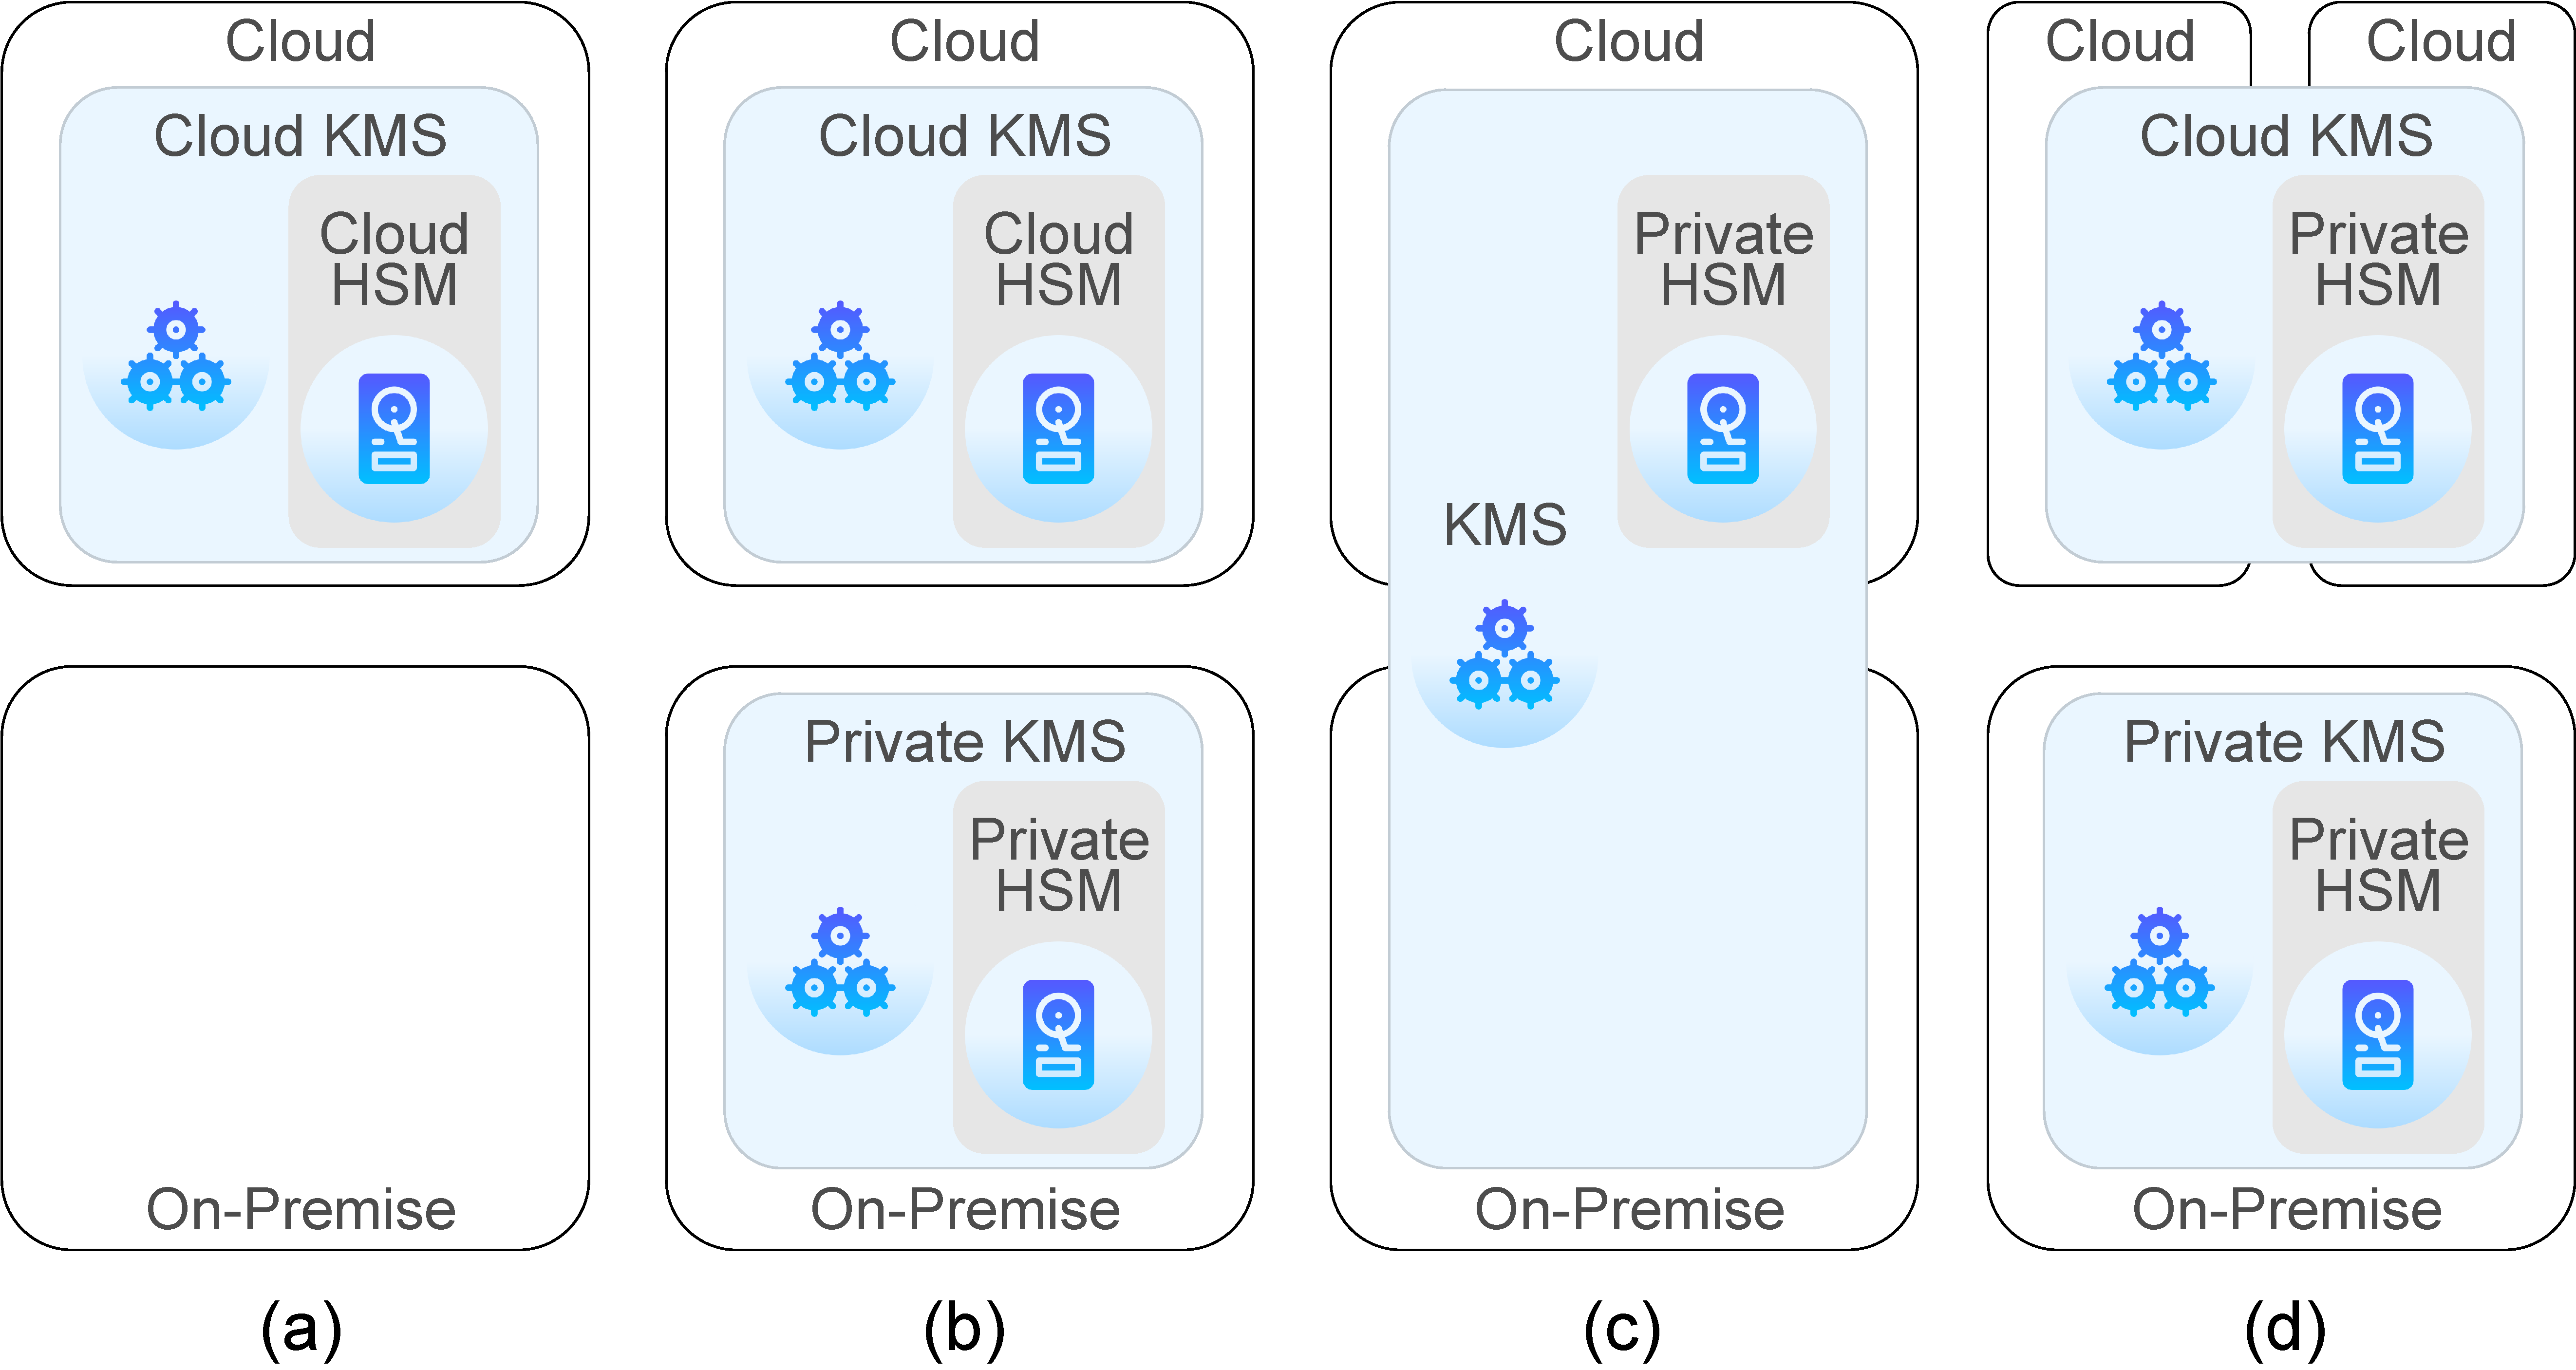
\includegraphics[width=1\linewidth]{resources/pdf/kms.pdf}
		\caption{\gls{kms} Architectures in the Cloud}
		\label{fig:kms}
	\end{center}
\end{figure}

As discussed in \cite{csa_key_2020} and shown in \Cref{fig:kms}, there are 4 main architectures with which an organization can interact with Cloud-based \glspl{kms}, which we discuss below (note that the use of \glspl{hsm} is strongly recommended in the context of \glspl{kms}). Intuitively, each architecture has its advantages and drawbacks, which organizations should carefully assess to identify the most suitable architecture for (the security, business, and regulatory requirements of) their scenarios. We report the properties of each architecture in \Cref{table:cloud_based_kms_architectures}, where a full, half, and empty circle (i.e., $\fullcirc$, $\halfcirc$, $\emptycirc$) mean that the corresponding property is fully achieved, partially achieved or not achieved by the corresponding architecture, respectively.

\begin{table}[!b]
	\centering
	\small
	\setlength{\tabcolsep}{1.75pt}
	\def\arraystretch{1.075}
	\rowcolors{0}{cloud}{white}
	\caption{Properties of Cloud-Based Key Management Systems Architectures}
	\newcolumntype{Y}{>{\centering\arraybackslash}X}
	\begin{tabularx}{\textwidth}{l|YYYY}
		
		\toprule
		
		\multicolumn{1}{c|}{\multirow{2}{*}\textbf{Property}} &
		\multicolumn{4}{c}\textbf{Cloud-based \gls{kms}} \\
		
		~ &
		\multicolumn{1}{c}\textbf{Pure} &
		\multicolumn{1}{c}\textbf{Combined} &
		\multicolumn{1}{c}\textbf{Hybrid} &
		\multicolumn{1}{c}\textbf{Multiple} \\
		
		\hline
		
		Transparency of the \gls{kms} 				& \emptycirc 	& \halfcirc 	& \fullcirc 	& \halfcirc 	\\
		Control over the \gls{kms} 					& \emptycirc 	& \halfcirc 	& \fullcirc 	& \halfcirc 	\\
		Portability (No Lock-In) 					& \emptycirc 	& \emptycirc 	& \fullcirc 	& \fullcirc 	\\
		Availability								& \halfcirc 	& \halfcirc 	& \halfcirc 	& \fullcirc 	\\
		Scalability									& \fullcirc 	& \fullcirc 	& \emptycirc 	& \fullcirc 	\\
		Performance									& \fullcirc 	& \fullcirc 	& \emptycirc 	& \fullcirc 	\\
		Interoperability with Other Cloud Providers & \emptycirc 	& \emptycirc 	& \emptycirc 	& \fullcirc 	\\
		Low Latency									& \fullcirc 	& \fullcirc 	& \emptycirc 	& \halfcirc 	\\
		Low Cost									& \fullcirc 	& \halfcirc 	& \emptycirc 	& \emptycirc 	\\
		Low Complexity (Fast Adoption)				& \fullcirc 	& \halfcirc 	& \emptycirc 	& \emptycirc 	\\
		Ease in Management							& \fullcirc 	& \halfcirc 	& \emptycirc 	& \emptycirc 	\\
		Prone to Satisfy Regulatory Requirements	& \emptycirc 	& \halfcirc 	& \fullcirc 	& \halfcirc 	\\
		Ease of SLA Definition and Enforcement		& \fullcirc 	& \halfcirc 	& \emptycirc 	& \halfcirc 	\\
		Seamless Support from Cloud Providers		& \fullcirc 	& \fullcirc 	& \halfcirc 	& \halfcirc 	\\
		Data Protection from Cloud Providers		& \emptycirc 	& \emptycirc 	& \fullcirc 	& \halfcirc 	\\
		Low Knowledge on \gls{kms} Required  		& \fullcirc 	& \halfcirc 	& \emptycirc 	& \emptycirc 	\\
		
		\bottomrule
		
	\end{tabularx}
	\label{table:cloud_based_kms_architectures}
\end{table}


% description
% advantages (``On the one hand'')
% disadvantages (``On the other hand'')
% when the architecture is recommended (``This architecture is usually recommended when'')
\paragraph*{Pure Cloud-Based Key Management System.}

\Cref{fig:kms}(a) shows an architecture where the \gls{kms} and the corresponding \gls{hsm} are managed entirely by a single Cloud provider --- ideally, the same provider offering the business services for which the \gls{kms} is used. The pure Cloud-based \gls{kms} is also known as ``Cloud-native \gls{kms}''. On the one hand, this architecture has intrinsically low latency, high performance, and high scalability, and it is the simplest to adopt, as it requires little knowledge on key management on the part of the organizations --- indeed, the Cloud provider manages all (or at least the majority of) aspects of the key management lifecycle. On the other hand, by delegating the \gls{kms} to the Cloud provider, organizations have little or no control over cryptographic keys (e.g., key lengths, cryptoperiod), cryptographic ciphers, or their configuration --- which may sometimes even be opaque to the organizations, complicating the achievement of compliance requirements. Moreover, (the design and functioning of) \gls{kms} offered by Cloud providers usually differ from each other, possibly leading to strong lock-in. This architecture is usually recommended when the organizations lack (or do not desire to acquire) specific expertise on \glspl{kms} and wish to achieve rapid deployment of business services \cite{csa_key_2020}. For a more detailed and concrete discussion on how to choose, plan, and deploy a pure Cloud-based \gls{kms} --- as well as technical, operational, regulatory, legal, and final recommendations --- we refer the interested reader to \cite{csa_recommendations_2021}.


\paragraph*{Combined Cloud-Based Key Management System.}

The architecture shown in \Cref{fig:kms}(b) extends the architecture in \Cref{fig:kms}(a) by allowing the exchange of cryptographic material between an on-premise \gls{kms} and a Cloud-based \gls{kms}; typically, cryptographic material (e.g., master keys) is created and exported from the former and then imported onto the latter --- it seldom happens the other way around \cite{csa_key_2020}. The two \glspl{kms} are thus distinct, that is, no integration is expected. The combined Cloud-based \gls{kms} is also known as ``Cloud-native \gls{kms} with an external key origin''. On the one hand, organizations have now some control over how cryptographic material is generated (e.g., what software and hardware are used). Moreover, this architecture has intrinsically low latency, high performance, high scalability, and little impact on \glspl{sla} with the Cloud provider. On the other hand, organizations are still limited by the design and functioning of Cloud-based \glspl{kms}, which requires organizations to configure the on-premise \gls{kms} (and private \gls{hsm}) to preserve compatibility --- while still entailing strong lock-in. Furthermore, organizations need some knowledge of \glspl{kms}. Finally, organizations should be aware of eventual modifications (e.g., addition of critical metadata) that Cloud providers apply on cryptographic material when imported on the Cloud-based \gls{kms} \cite{csa_key_2020} --- hence, transparency is still limited.\footnote{Service encryption with Microsoft Purview Customer Key (\url{https://docs.microsoft.com/en-us/microsoft-365/compliance/customer-key-overview?view=o365-worldwide})} This architecture is usually recommended when organizations want to control (at least the) the generation of cryptographic material or need to fulfill specific regulatory requirements that cannot be achieved by using Cloud-based \gls{kms} only --- such as \gls{byok} (see \Cref{sec:cloud:models}). For a more detailed and concrete discussion on how to choose, plan, and deploy a combined Cloud-based \gls{kms} --- as well as technical, operational, regulatory, legal, and final recommendations --- we refer the interested reader to \cite{csa_recommendations_2021_2}.


\paragraph*{Hybrid Cloud-Based Key Management System.}

The architecture in \Cref{fig:kms}(c) shows a \gls{kms} logically spanning from the organization on-premise to the Cloud provider; in other words, functions of the \gls{kms} are used from both on-premise and the Cloud. This architecture follows either the ``Bring-Your-Own-\gls{hsm}'' or the ``\gls{hsm}-as-a-Service'' models:\footnote{The \gls{cla} --- a not-for-profit organization with the mission to educate and promote the use of best practices for security in the Cloud --- is currently working (November 2023) on a white paper tentatively entitled ``\gls{hsm}-as-a-Service: Use Cases, Considerations, and Best Practices''; for more information, see \url{https://cloudsecurityalliance.org/artifacts/hsm-as-a-service-use-cases-considerations-and-best-practices/}} the former means that an organization provides a physical \gls{hsm} that is hosted in the Cloud, while the latter means that the Cloud provider provisions an \gls{hsm} solely for use by the organization \cite{csa_key_2020}. The hybrid Cloud-based \gls{kms} is also known as ``Cloud-native \gls{kms} using external \glspl{kms}''. On the one hand, organizations have full control over the \gls{kms}, the key management lifecycle, and its configuration (recall the concepts explained in \Cref{sec:key_management}) while preventing strong lock-in. On the other hand, this architecture has high cost and limited performance, scalability, and latency. Moreover, this architecture requires the (often complex) definition of \glspl{sla} with the Cloud provider on the use of the \gls{kms} and the \gls{hsm} --- especially in case of incidents. Furthermore, organizations need deep knowledge of \glspl{kms}. This architecture is usually recommended when organizations want full control over the \gls{kms}, need to fulfill specific regulatory requirements that cannot be achieved by adopting other architectures --- such as \gls{cyok} (see \Cref{sec:cloud:models}) --- or must protect their data even from Cloud providers themselves (see \Cref{sec:cloud:models}). As a final remark, note that this architecture is not always supported by Cloud providers (e.g., in 2020, only \gls{aws} and Microsoft provided support for this architecture \cite{csa_key_2020}). For a more detailed and concrete discussion on how to choose, plan, and deploy a hybrid Cloud-based \gls{kms} --- as well as technical, operational, regulatory, legal, and final recommendations --- we refer the interested reader to \cite{csa_recommendations_2022}.


\paragraph*{Multiple Cloud-Based Key Management System.}

The architecture shown in \Cref{fig:kms}(d) illustrated a combined \gls{kms} where the Cloud-based \gls{kms} spans two or more Cloud providers. The multiple Cloud-based \gls{kms} is also known as ``Multi-Cloud \glspl{kms}''. On the one hand, this architecture provides high portability, fault tolerance, and scalability --- mainly due to the use of several Cloud providers. On the other hand, organizations need both deep knowledge of both \glspl{kms} and their functioning as offered by multiple Cloud providers. Also, the complexity of the architecture entails higher costs due to longer design and deployment time. This architecture is usually recommended when the business services of organizations already span multiple Cloud providers, or if organizations need to satisfy specific and complex regulatory requirements. 



\subsubsection{Cloud Providers Offering Key Management Systems Services}\label{sec:cloud:providers}

The first Cloud-based \gls{kms} service was the \gls{aws} Key Management Service, released in late 2014.\footnote{Document history - AWS Key Management Service (\url{https://docs.aws.amazon.com/kms/latest/developerguide/dochistory.html})} Since then, many other Cloud providers implemented and released \glspl{kms}, making proper \glspl{sdk} readily available to organizations. Below, we briefly describe Cloud-based \glspl{kms} and related services offered by 3 major Cloud providers, namely \gls{aws}, Google, and Microsoft.

\remarkBlock{Change velocity of cloud-based \glspl{kms}}{Cloud computing is known for its fast pacing and rapid evolution of products and services; intuitively, this characteristic applies to Cloud-based \glspl{kms} and related services as well. In other words, these often change, and it is therefore recommended to refer to the latest documentation for complete, accurate, and updated information. The content of \Cref{sec:cloud:providers} --- which is to be intended as an overview --- is updated as of December 2023.}


\paragraph*{Amazon Web Services.}

\gls{aws} offers two main services related to Cloud-based \gls{kms}:

\begin{itemize}
	\item \textbf{\gls{aws} Key Management Service}\footnote{Encryption Cryptography Signing - AWS Key Management Service (\url{https://aws.amazon.com/kms/})}: a managed service allowing organizations to handle the key management lifecycle (see \Cref{sec:key_management}) using \glspl{hsm} certified under \gls{fips} 140-2 level 3 (see \Cref{sec:hardware}). The \gls{aws} Key Management Service integrates with most other \gls{aws} services, such as \gls{aws} \gls{s3} --- for encryption of data at rest --- \gls{aws} \gls{iam} --- for authentication and authorization through the definition and enforcement of fine-grained \gls{abac} policies --- and \gls{aws} CloudTrail\footnote{Api Logs - AWS CloudTrail (\url{https://aws.amazon.com/cloudtrail/})} --- for monitoring and auditing key usages. Finally, the \gls{aws} Key Management Service allows organizations to import cryptographic material and synchronize with external \gls{hsm} (i.e., combined Cloud-based \gls{kms}, as discussed in \Cref{sec:cloud:architectures});
	\item \textbf{\gls{aws} CloudHSM}\footnote{Security HSM - AWS CloudHSM (\url{https://aws.amazon.com/cloudhsm/})}: a managed service offering \glspl{hsm}-as-a-Service (recall the corresponding definition in \Cref{sec:cloud:architectures}), employing \glspl{hsm} certified under \gls{fips} 140-2 level 3. CloudHSM allows organizations to manage cryptographic keys --- accessible only by the organizations themselves --- by creating a cluster of \glspl{hsm} spread across multiple \gls{aws} availability zones in a region for high availability and automatic load balancing. CloudHSM does not interoperate directly with on-premises \glspl{hsm}.
\end{itemize}

The Custom Key Store feature\footnote{Custom key stores - AWS Key Management Service (\url{https://docs.aws.amazon.com/kms/latest/developerguide/custom-key-store-overview.html})} combines the controls provided by CloudHSM with the integration and ease of use of the \gls{aws} Key Management Service. In other words, an organization can configure its CloudHSM cluster and then use it from the \gls{aws} Key Management Service as a dedicated key store for keys rather than the default key store. Intuitively, the organization is then responsible for the key management lifecycle of keys generated within the CloudHSM cluster (e.g., key rotation should be performed manually).


\paragraph*{Google.}

Google offers two main services related to Cloud-based \gls{kms} in the Google Cloud suite of Cloud Services:

\begin{itemize}
	\item \textbf{Cloud Key Management Service}:\footnote{Cloud Key Management Service overview | Cloud KMS Documentation (\url{https://cloud.google.com/kms/docs/key-management-service})} a managed service allowing organizations to handle the key management lifecycle (see \Cref{sec:key_management}) using either software-based cryptographic modules certified under \gls{fips} 140-2 level 1 or \glspl{hsm} certified under \gls{fips} 140-2 level 3 with Google Cloud \gls{hsm}.\footnote{Cloud HSM | Cloud KMS Documentation (\url{https://cloud.google.com/kms/docs/hsm})} The Cloud Key Management Service integrates with most other Google Cloud services, such as Cloud \gls{iam}\footnote{Identity and Access Management | IAM | Google Cloud (\url{https://cloud.google.com/iam})} --- for authentication and authorization through the definition and enforcement of fine-grained \gls{abac} policies --- and Cloud Audit Logging\footnote{Cloud Audit Logs overview (\url{https://cloud.google.com/logging/docs/audit})} --- for monitoring and auditing key usages; encryption for data at rest is enabled by default. Finally, the Cloud Key Management Service allows organizations to import cryptographic material and synchronize with external \gls{hsm} (i.e., combined Cloud-based \gls{kms}, as discussed in \Cref{sec:cloud:architectures});
	\item \textbf{Cloud \gls{ekm}}:\footnote{Cloud External Key Manager | Cloud KMS Documentation (\url{https://cloud.google.com/kms/docs/ekm})} a managed service --- released in early access in September 2023 --- allowing to indirectly use cryptographic keys managed by an external \gls{kms} in Google Cloud services (i.e., similar to the combined Cloud-based \gls{kms}, as discussed in \Cref{sec:cloud:architectures}). In other words, keys are never used, cached, or stored within the Google Cloud services, and instead Cloud \gls{ekm} directly invokes the \glspl{api} of the external \gls{kms} --- as it happens in \gls{hyok} models (see \Cref{sec:cloud:models}). This implies that data is always encrypted before being sent to the Cloud, while decryption of data always happens within the external \gls{kms}.
\end{itemize}


\paragraph*{Microsoft Azure.}

Microsoft offers two main services related to Cloud-based \gls{kms} in the Azure Cloud platform:

\begin{itemize}
	\item \textbf{Key Vault}\footnote{Key Vault | Microsoft Azure (\url{https://azure.microsoft.com/en-us/products/key-vault})}: a managed service for the management of generic secrets --- hence, also cryptographic keys. Key Vault has two service tiers: standard, which encrypts with a software key, and premium, which includes the use of \glspl{hsm} certified under \gls{fips} 140-2 level 3;
	\item \textbf{Azure Managed, Dedicated, and Payment \gls{hsm}}\footnote{Overview of Key Management in Azure | Microsoft Learn (\url{https://learn.microsoft.com/en-us/azure/security/fundamentals/key-management})}: a set of 3 managed services offering \glspl{hsm}-as-a-Service (recall the corresponding definition in \Cref{sec:cloud:architectures}), employing \glspl{hsm} certified under FIPS 140-2 level 3. Azure Managed \gls{hsm} is managed by Azure, while the organization is responsible for Azure Dedicated and Payment \gls{hsm}; Azure Dedicated \gls{hsm} is general purpose, while Azure Payment \gls{hsm} is specific for applications in financial services.\footnote{How to choose the right key management solution - How to choose between Azure Key Vault, Azure Managed HSM, Azure Dedicated HSM, and Azure Payment HSM | Microsoft Learn (\url{https://learn.microsoft.com/en-us/azure/security/fundamentals/key-management-choose})}
\end{itemize}

In summary, all 3 Cloud providers offer services related to Cloud-based \gls{kms}. However, \gls{aws} and Google seem to have the most articulated and consolidated services, while Microsoft still lacks a complete \gls{kms}. Note that all 3 Cloud providers claim that no one, including their employees, can retrieve keys from \glspl{hsm}: this may be reasonable by considering that Cloud providers are motivated to avoid legal and reputational damages associated with unauthorized data access and voluntarily allow inspections by third-party auditors.\footnote{Cloud encryption key management: how can Swiss organizations protect their data outside their premises? (\url{https://www2.deloitte.com/ch/en/pages/technology/articles/cloud-encryption-key-management.html})}



\subsubsection{Key Management Models for the Cloud}\label{sec:cloud:models}

As discussed in \Cref{sec:cloud:architectures,sec:cloud:providers}, cryptographic keys can be managed (e.g., generated, used) differently depending on the chosen Cloud-based \glspl{kms} architecture and \gls{kms} Cloud service. In particular, we identify 3 relevant aspects in this regard: ownership, control, and possession --- which correspond to who owns, controls the lifecycle, and physically keeps cryptographic keys (and data, in general). Although ownership of keys is always of the organization (i.e., the customer of the Cloud for which the keys were created), the level of control and possession may vary. For this reason, in the last years, 3 key management models for the Cloud emerged, based on how organizations manage (some aspects of) the key management lifecycle (e.g., generation) externally with respect to Cloud-based \gls{kms} and related services (e.g., using an on-premise \gls{kms} with a dedicated \gls{hsm}):

\begin{itemize}
	\item \textbf{\gls{byok}}: in this model (often also called ``customer-supplied encryption keys''), keys are generated by organizations and imported onto the Cloud for use --- as it happens in the combined Cloud-based \gls{kms} architecture (see \Cref{sec:cloud:architectures}) --- resulting in seamless integration with Cloud services but also the loss of ownership over the keys. Indeed, in \gls{byok}, the Cloud provider has access to private and secret keys;
	\item \textbf{\gls{cyok}}: in this model, keys are generated by organizations and imported onto the Cloud for use --- as it happens in the hybrid Cloud-based \gls{kms} architecture(see \Cref{sec:cloud:architectures}). Although in \gls{byok} cryptographic keys reside within the Cloud, the Cloud provider has no access to private and secret keys (at least theoretically);
	\item \textbf{\gls{hyok}}: in this model, organizations retain full control and ownership over keys, which are never used, cached, or stored in the Cloud (e.g., as it happens in the Cloud \gls{ekm} described in \Cref{sec:cloud:providers}).
\end{itemize}

As is usually the case, there is no key management model that is the most suitable for (the security, business, and regulatory requirements of) all scenarios. Instead, the choice of which model to adopt should be taken on a case-by-case basis. For instance, for most Cloud services following the \gls{saas} pattern (e.g., emails, managed database, analytics services), the Cloud provider must have access to plaintext data; therefore, the \gls{cyok} and \gls{hyok} models are hardly compatible with \gls{saas} services. On the other hand, if an organization requires to preserve the confidentiality of its data even with respect to the Cloud provider, the \gls{byok} model may not be a suitable choice --- especially when combined with dedicated cryptographic constructions such as \gls{cac} \cite{berlato_formal_2022,berlato_end_2022}. Other aspects to consider are further regulatory and compliance requirements, existing key management practices, and the level of control and visibility for keys desired by organizations.

\remarkBlock{Debate around key management models for the cloud}{The acronyms \gls{byok}, \gls{cyok}, and \gls{hyok} originated first as marketing terms and, at the time of writing, there is no official standard or widely agreed upon definition for their semantics; therefore, some deem these terms --- and, in particular, their use --- to be pointless or even confusing, and suggest instead to avoid them entirely \cite{csa_key_2020}.}




* add transparency logs into popular applications examples

wireguard VPN
% vedi nel progetto CC la deliverable R3-CSC-D1-def

